        %%******************************************%%
        %%                                          %%
        %%        Modello di tesi di laurea         %%
        %%            di Andrea Giraldin            %%
        %%                                          %%
        %%             2 novembre 2012              %%
        %%                                          %%
        %%******************************************%%


% I seguenti commenti speciali impostano:
% 1. 
% 2. PDFLaTeX come motore di composizione;
% 3. tesi.tex come documento principale;
% 4. il controllo ortografico italiano per l'editor.

% !TEX encoding = UTF-8
% !TEX TS-program = pdflatex
% !TEX root = tesi.tex
% !TEX spellcheck = it-IT

% PDF/A filecontents
\RequirePackage{filecontents}
\begin{filecontents*}{\jobname.xmpdata}
  \Title{Document’s title}
  \Author{Author’s name}
  \Language{it-IT}
  \Subject{The abstract, or short description.}
  \Keywords{keyword1\sep keyword2\sep keyword3}
\end{filecontents*}

\documentclass[10pt,                    % corpo del font principale
               a4paper,                 % carta A4
               twoside,                 % impagina per fronte-retro
               openright,               % inizio capitoli a destra
               english,                 
               italian,                 
               ]{book}    

%**************************************************************
% Importazione package
%************************************************************** 

\PassOptionsToPackage{dvipsnames}{xcolor} % colori PDF/A
%\usepackage[dvipsnames]{xcolor}

\usepackage{colorprofiles}

\usepackage[a-2b,mathxmp]{pdfx}[2018/12/22]
                                        % configurazione PDF/A
                                        % validare in https://www.pdf-online.com/osa/validate.aspx

%\usepackage{amsmath,amssymb,amsthm}    % matematica

%\usepackage[T1]{fontenc}                % codifica dei font:
                                        % NOTA BENE! richiede una distribuzione *completa* di LaTeX

\usepackage[utf8]{inputenc}             % codifica di input; anche [latin1] va bene
                                        % NOTA BENE! va accordata con le preferenze dell'editor

\usepackage[english, italian]{babel}    % per scrivere in italiano e in inglese;
                                        % l'ultima lingua (l'italiano) risulta predefinita

\usepackage{bookmark}                   % segnalibri

\usepackage{caption}                    % didascalie

\usepackage{chngpage,calc}              % centra il frontespizio

\usepackage{comment}

\usepackage{csquotes}                   % gestisce automaticamente i caratteri (")

\usepackage{emptypage}                  % pagine vuote senza testatina e piede di pagina

\usepackage{epigraph}			% per epigrafi

\usepackage{eurosym}                    % simbolo dell'euro

%\usepackage{indentfirst}               % rientra il primo paragrafo di ogni sezione

\usepackage{graphicx}                   % immagini

\usepackage{hyperref}                   % collegamenti ipertestuali

\usepackage[binding=5mm]{layaureo}      % margini ottimizzati per l'A4; rilegatura di 5 mm

\usepackage{listings}                   % codici

\usepackage{microtype}                  % microtipografia

\usepackage{mparhack,fixltx2e,relsize}  % finezze tipografiche

\usepackage{nameref}                    % visualizza nome dei riferimenti                                      
\usepackage[font=small]{quoting}        % citazioni

\usepackage{subfig}                     % sottofigure, sottotabelle

\usepackage[italian]{varioref}          % riferimenti completi della pagina

\usepackage{booktabs}                   % tabelle                                       
\usepackage{tabularx}                   % tabelle di larghezza prefissata                                    
\usepackage{longtable}                  % tabelle su più pagine                                        
\usepackage{ltxtable}                   % tabelle su più pagine e adattabili in larghezza


\newcolumntype{C}[1]{>{\centering\let\newline\\\arraybackslash\hspace{0pt}}m{#1}}
\newcolumntype{R}[1]{>{\raggedleft\let\newline\\\arraybackslash\hspace{0pt}}m{#1}}
\newcolumntype{L}[1]{>{\raggedright\let\newline\\\arraybackslash\hspace{0pt}}m{#1}}

\definecolor{mongogreen}{HTML}{A0C080}


\usepackage[toc, acronym]{glossaries}   % glossario
                                        % per includerlo nel documento bisogna:
                                        % 1. compilare una prima volta tesi.tex;
                                        % 2. eseguire: makeindex -s tesi.ist -t tesi.glg -o tesi.gls tesi.glo
                                        % 3. eseguire: makeindex -s tesi.ist -t tesi.alg -o tesi.acr tesi.acn
                                        % 4. compilare due volte tesi.tex.

\usepackage[backend=biber,style=verbose-ibid,hyperref,backref]{biblatex}
                                        % eccellente pacchetto per la bibliografia; 
                                        % produce uno stile di citazione autore-anno; 
                                        % lo stile "numeric-comp" produce riferimenti numerici
                                        % per includerlo nel documento bisogna:
                                        % 1. compilare una prima volta tesi.tex;
                                        % 2. eseguire: biber tesi
                                        % 3. compilare ancora tesi.tex.

%**************************************************************
% file contenente le impostazioni della tesi
%**************************************************************

%**************************************************************
% Frontespizio
%**************************************************************

% Autore
\newcommand{\myName}{Nicholas Sertori}                                    
\newcommand{\myTitle}{Realizzazione e analisi prestazionale di un database NoSQL per la possibile migrazione da un database relazionale}

% Tipo di tesi                   
\newcommand{\myDegree}{Tesi di laurea}

% Università             
\newcommand{\myUni}{Università degli Studi di Padova}

% Facoltà       
\newcommand{\myFaculty}{Corso di Laurea in Informatica}

% Dipartimento
\newcommand{\myDepartment}{Dipartimento di Matematica ``Tullio Levi-Civita''}

% Titolo del relatore
\newcommand{\profTitle}{Prof. }

% Relatore
\newcommand{\myProf}{Luigi De Giovanni}

% Luogo
\newcommand{\myLocation}{Padova}

% Anno accademico
\newcommand{\myAA}{2021-2022}

% Data discussione
\newcommand{\myTime}{Dicembre 2022}

% Matricola
\newcommand{\myMatricola}{1193171}

%**************************************************************
% Impostazioni di impaginazione
% see: http://wwwcdf.pd.infn.it/AppuntiLinux/a2547.htm
%**************************************************************

\setlength{\parindent}{14pt}   % larghezza rientro della prima riga
\setlength{\parskip}{0pt}   % distanza tra i paragrafi


%**************************************************************
% Impostazioni di biblatex
%**************************************************************
\bibliography{bibliografia} % database di biblatex 

\defbibheading{bibliography} {
    \cleardoublepage
    \phantomsection 
    \addcontentsline{toc}{chapter}{\bibname}
    \chapter*{\bibname\markboth{\bibname}{\bibname}}
}

\setlength\bibitemsep{1.5\itemsep} % spazio tra entry

\DeclareBibliographyCategory{opere}
\DeclareBibliographyCategory{web}

\addtocategory{opere}{womak:lean-thinking}
\addtocategory{web}{site:agile-manifesto}

\defbibheading{opere}{\section*{Riferimenti bibliografici}}
\defbibheading{web}{\section*{Siti Web consultati}}


%**************************************************************
% Impostazioni di caption
%**************************************************************
\captionsetup{
    tableposition=top,
    figureposition=bottom,
    font=small,
    format=hang,
    labelfont=bf
}

%**************************************************************
% Impostazioni di glossaries
%**************************************************************
\makeglossaries

%**************************************************************
% Glossario
%**************************************************************

\newglossaryentry{DAO}
{
    name=DAO,
    description={}
}

\newglossaryentry{database distribuito}
{
    name=database distribuito,
    description={}
}

\newglossaryentry{DBaaS}
{
    name=DBaaS,
    description={}
}

\newglossaryentry{DTO}
{
    name=DTO,
    description={}
}

\newglossaryentry{EclipseLink}
{
    name=EclipseLink,
    description={}
}


\newglossaryentry{Hybernate}
{
    name=Hybernate,
    description={}
}


\newglossaryentry{JDBC}
{
    name=JDBC,
    description={}
}

\newglossaryentry{JPA}
{
    name=JPA,
    description={}
}

\newglossaryentry{KPI}
{
    name=KPI,
    description={}
}

\newglossaryentry{master-slave}
{
    name=master-slave,
    description={}
}

\newglossaryentry{Model-View-ViewModel}
{
    name=Model-View-ViewModel,
    description={}
}

\newglossaryentry{rest API}
{
    name=rest API,
    description={}
}

\newglossaryentry{SQL}
{
    name=SQL,
    description={}
}

\newglossaryentry{test di carico}
{
    name=test di carico,
    description={}
}

\newglossaryentry{Tomcat}
{
    name=Tomcat,
    description={}
}

 % database di termini


%**************************************************************
% Impostazioni di graphicx
%**************************************************************
\graphicspath{{immagini/}} % cartella dove sono riposte le immagini


%**************************************************************
% Impostazioni di hyperref
%**************************************************************
\definecolor{bluelink}{HTML}{0299C1}
\definecolor{purplink}{HTML}{44018D}

\hypersetup{
    %hyperfootnotes=false,
    %pdfpagelabels,
    %draft,	% = elimina tutti i link (utile per stampe in bianco e nero)
    colorlinks=true,
    linktocpage=true,
    pdfstartpage=1,
    pdfstartview=,
    % decommenta la riga seguente per avere link in nero (per esempio per la stampa in bianco e nero)
    %colorlinks=false, linktocpage=false, pdfborder={0 0 0}, pdfstartpage=1, pdfstartview=FitV,
    breaklinks=true,
    pdfpagemode=UseNone,
    pageanchor=true,
    pdfpagemode=UseOutlines,
    plainpages=false,
    bookmarksnumbered,
    bookmarksopen=true,
    bookmarksopenlevel=1,
    hypertexnames=true,
    pdfhighlight=/O,
    %nesting=true,
    %frenchlinks,
    urlcolor=webbrown,
    %linkcolor=RoyalBlue,
    linkcolor=bluelink,
    citecolor=Black,
    %citecolor=webgreen,
    %pagecolor=RoyalBlue,
    %urlcolor=Black, linkcolor=Black, citecolor=Black, %pagecolor=Black,
    pdftitle={\myTitle},
    pdfauthor={\textcopyright\ \myName, \myUni, \myFaculty},
    pdfsubject={},
    pdfkeywords={},
    pdfcreator={pdfLaTeX},
    pdfproducer={LaTeX}
}

%**************************************************************
% Impostazioni di itemize
%**************************************************************
\renewcommand{\labelitemi}{$\ast$}

%\renewcommand{\labelitemi}{$\bullet$}
%\renewcommand{\labelitemii}{$\cdot$}
%\renewcommand{\labelitemiii}{$\diamond$}
%\renewcommand{\labelitemiv}{$\ast$}


%**************************************************************
% Impostazioni di listings
%**************************************************************
\lstset{
    language=[LaTeX]Tex,%C++,
    keywordstyle=\color{RoyalBlue}, %\bfseries,
    basicstyle=\small\ttfamily,
    %identifierstyle=\color{NavyBlue},
    commentstyle=\color{Green}\ttfamily,
    stringstyle=\rmfamily,
    numbers=none, %left,%
    numberstyle=\scriptsize, %\tiny
    stepnumber=5,
    numbersep=8pt,
    showstringspaces=false,
    breaklines=true,
    frameround=ftff,
    frame=single
} 


%**************************************************************
% Impostazioni di xcolor
%**************************************************************
\definecolor{webgreen}{rgb}{0,.5,0}
\definecolor{webbrown}{rgb}{.6,0,0}

%**************************************************************
% Altro
%**************************************************************

\newcommand{\omissis}{[\dots\negthinspace]} % produce [...]

% eccezioni all'algoritmo di sillabazione
\hyphenation
{
    ma-cro-istru-zio-ne
    gi-ral-din
}

\newcommand{\sectionname}{Sezione}
\addto\captionsitalian{\renewcommand{\figurename}{Figura}
                       \renewcommand{\tablename}{Tabella}}

\newcommand{\glsfirstoccur}{\ap{{[g]}}}

\newcommand{\intro}[1]{\emph{\textsf{#1}}}

%**************************************************************
% Environment per ``rischi''
%**************************************************************
\newcounter{riskcounter}                % define a counter
\setcounter{riskcounter}{0}             % set the counter to some initial value

%%%% Parameters
% #1: Title
\newenvironment{risk}[1]{
    \refstepcounter{riskcounter}        % increment counter
    \par \noindent                      % start new paragraph
    \textbf{\arabic{riskcounter}. #1}   % display the title before the 
                                        % content of the environment is displayed 
}{
    \par\medskip
}

\newcommand{\riskname}{Rischio}

\newcommand{\riskdescription}[1]{\textbf{\\Descrizione:} #1.}

\newcommand{\risksolution}[1]{\textbf{\\Soluzione:} #1.}

%**************************************************************
% Environment per ``use case''
%**************************************************************
\newcounter{usecasecounter}             % define a counter
\setcounter{usecasecounter}{0}          % set the counter to some initial value

%%%% Parameters
% #1: ID
% #2: Nome
\newenvironment{usecase}[2]{
    \renewcommand{\theusecasecounter}{\usecasename #1}  % this is where the display of 
                                                        % the counter is overwritten/modified
    \refstepcounter{usecasecounter}             % increment counter
    \vspace{10pt}
    \par \noindent                              % start new paragraph
    {\large \textbf{\usecasename #1: #2}}       % display the title before the 
                                                % content of the environment is displayed 
    \medskip
}{
    \medskip
}

\newcommand{\usecasename}{UC}

\newcommand{\usecaseactors}[1]{\textbf{\\Attori Principali:} #1. \vspace{4pt}}
\newcommand{\usecasepre}[1]{\textbf{\\Precondizioni:} #1. \vspace{4pt}}
\newcommand{\usecasedesc}[1]{\textbf{\\Descrizione:} #1. \vspace{4pt}}
\newcommand{\usecasepost}[1]{\textbf{\\Postcondizioni:} #1. \vspace{4pt}}
\newcommand{\usecasealt}[1]{\textbf{\\Scenario Alternativo:} #1. \vspace{4pt}}

%**************************************************************
% Environment per ``namespace description''
%**************************************************************

\newenvironment{namespacedesc}{
    \vspace{10pt}
    \par \noindent                              % start new paragraph
    \begin{description} 
}{
    \end{description}
    \medskip
}

\newcommand{\classdesc}[2]{\item[\textbf{#1:}] #2}
                     % file con le impostazioni personali

\begin{document}
%**************************************************************
% Materiale iniziale
%**************************************************************
\frontmatter
% !TEX encoding = UTF-8
% !TEX TS-program = pdflatex
% !TEX root = ../tesi.tex

%**************************************************************
% Frontespizio 
%**************************************************************
\begin{titlepage}

\begin{center}

\begin{LARGE}
\textbf{\myUni}\\
\end{LARGE}

\vspace{10pt}

\begin{Large}
\textsc{\myDepartment}\\
\end{Large}

\vspace{10pt}

\begin{large}
\textsc{\myFaculty}\\
\end{large}

\vspace{30pt}
\begin{figure}[htbp]
\begin{center}

\includegraphics[height=6cm]{logo-unipd}
\end{center}
\end{figure}
\vspace{30pt} 

\begin{LARGE}
\begin{center}
\textbf{\myTitle}\\
\end{center}
\end{LARGE}

\vspace{10pt} 

\begin{large}
\textsl{\myDegree}\\
\end{large}

\vspace{40pt} 

\begin{large}
\begin{flushleft}
\textit{Relatore}\\ 
\vspace{5pt} 
\profTitle \myProf
\end{flushleft}

\vspace{0pt} 

\begin{flushright}
\textit{Laureando}\\ 
\vspace{5pt} 
\myName
\end{flushright}
\end{large}

\vspace{40pt}

\line(1, 0){338} \\
\begin{normalsize}
\textsc{Anno Accademico \myAA}
\end{normalsize}

\end{center}
\end{titlepage} 
% !TEX encoding = UTF-8
% !TEX TS-program = pdflatex
% !TEX root = ../tesi.tex

%**************************************************************
% Colophon
%**************************************************************
\clearpage
\phantomsection
\thispagestyle{empty}

\hfill

\vfill

\noindent\myName: \textit{\myTitle,}
\myDegree,
\textcopyright\ \myTime.
% !TEX encoding = UTF-8
% !TEX TS-program = pdflatex
% !TEX root = ../tesi.tex

%**************************************************************
% Dedica
%**************************************************************
\cleardoublepage
\phantomsection
\thispagestyle{empty}
\pdfbookmark{Dedica}{Dedica}

\vspace*{3cm}

\begin{center}
Lorem ipsum dolor sit amet, consectetuer adipiscing elit. \\ \medskip
--- Oscar Wilde    
\end{center}

\medskip

\begin{center}
Dedicato a ...
\end{center}

% !TEX encoding = UTF-8
% !TEX TS-program = pdflatex
% !TEX root = ../tesi.tex

%**************************************************************
% Sommario
%**************************************************************
\cleardoublepage
\phantomsection
\pdfbookmark{Sommario}{Sommario}
\begingroup
\let\clearpage\relax
\let\cleardoublepage\relax
\let\cleardoublepage\relax

\chapter*{Sommario}

Il presente documento descrive il lavoro svolto durante il periodo di stage svolto presso l'azienda Ifin Sistemi s.r.l. Lo stage è stato svolto alla conclusione del percorso di studi della laurea triennale in Informatica, occupando circa trecentoventi ore divise in otto settimane.
Lo scopo del progetto svolto è stato di effettuare uno studio di fattibilità per l’integrazione di una soluzione di database NoSQL nei prodotti dell'azienda. Lo studio di fattibilità ha comportato una fase di analisi delle varie soluzioni NoSQL esistenti sul mercato, una fase di analisi delle soluzioni attualmente adottate all'interno dei prodotti Ifin, ed infine una fase di valutazione pratica delle soluzioni individuate, con relativi benchmark per il confronto delle prestazioni ed un approfondimento sulle differenze di progettazione tra database relazionali classici e database NoSQL.

%\vfill
%
%\selectlanguage{english}
%\pdfbookmark{Abstract}{Abstract}
%\chapter*{Abstract}
%
%\selectlanguage{italian}

\endgroup			

\vfill


% !TEX encoding = UTF-8
% !TEX TS-program = pdflatex
% !TEX root = ../tesi.tex

%**************************************************************
% Ringraziamenti
%**************************************************************
\cleardoublepage
\phantomsection
\pdfbookmark{Ringraziamenti}{ringraziamenti}

\begin{flushright}{
	\slshape    
	``Life is really simple, but we insist on making it complicated''} \\ 
	\medskip
    --- Confucius
\end{flushright}


\bigskip

\begingroup
\let\clearpage\relax
\let\cleardoublepage\relax
\let\cleardoublepage\relax

\chapter*{Ringraziamenti}

\noindent \textit{Innanzitutto, vorrei esprimere la mia gratitudine al Prof. NomeDelProfessore, relatore della mia tesi, per l'aiuto e il sostegno fornitomi durante la stesura del lavoro.}\\

\noindent \textit{Desidero ringraziare con affetto i miei genitori per il sostegno, il grande aiuto e per essermi stati vicini in ogni momento durante gli anni di studio.}\\

\noindent \textit{Ho desiderio di ringraziare poi i miei amici per tutti i bellissimi anni passati insieme e le mille avventure vissute.}\\
\bigskip

\noindent\textit{\myLocation, \myTime}
\hfill \myName

\endgroup


% !TEX encoding = UTF-8
% !TEX TS-program = pdflatex
% !TEX root = ../tesi.tex

%**************************************************************
% Indici
%**************************************************************
\cleardoublepage
\pdfbookmark{\contentsname}{tableofcontents}
\setcounter{tocdepth}{2}
\tableofcontents
%\markboth{\contentsname}{\contentsname} 
\clearpage

\begingroup 
    \let\clearpage\relax
    \let\cleardoublepage\relax
    \let\cleardoublepage\relax
    %*******************************************************
    % Elenco delle figure
    %*******************************************************    
    \phantomsection
    \pdfbookmark{\listfigurename}{lof}
    \listoffigures

    \vspace*{8ex}

    %*******************************************************
    % Elenco delle tabelle
    %*******************************************************
    \phantomsection
    \pdfbookmark{\listtablename}{lot}
    \listoftables
        
    \vspace*{8ex}
\endgroup

\cleardoublepage

\cleardoublepage

%**************************************************************
% Materiale principale
%**************************************************************
\mainmatter
% !TEX encoding = UTF-8
% !TEX TS-program = pdflatex
% !TEX root = ../tesi.tex

%**************************************************************
\chapter{Introduzione}
\label{cap:introduzione}

%**************************************************************
\section{L'azienda}

L'azienda proponente è Ifin Sistemi s.r.l., un'azienda di prodotto che si occupa principalmente di informatica finanziaria (logo in \autoref{fig:ifin}).
Il suo \textit{core business} è incentrato su piattaforme che facilitano l'archiviazione di pratiche e documenti legali in modo sicuro e affidabile, e mediano l'invio di fatture elettroniche tra aziende e Sistema di Interscambio, un sistema informatico gestito dall'Agenzia delle Entrate.

\vspace{15pt}
\begin{figure}[htbp]
\begin{center}

\includegraphics[height=3cm]{logo-ifin}
\caption{Logo di Ifin Sistemi s.r.l.}
\label{fig:ifin}
\end{center}
\end{figure}
\vspace{15pt}

%**************************************************************
\section{Situazione attuale}

I due prodotti di punta dell'azienda, che compongono il \textit{core business} sopra accennato, sono \textit{LegalArchive} e \textit{InvoiceChannel}. All'interno di Ifin, coesistono vari team che mantengono la codebase di questi software, occupandosi della loro manutenzione e della modellazione di nuove funzionalità richieste dai clienti.\\
A livello pratico, il codice per i software di Ifin è scritto in \textit{Java}, appoggiato quando serve al framework \textit{Spring}.\\
All'interno di quello che è lo stack tecnologico aziendale, data la scelta del linguaggio di programmazione, si trova quello che può essere considerato uno standard per lo sviluppo di applicativi che fanno largo uso di database. Tecnologie come \gls{JPA}\ped{G}, \gls{JDBC}\ped{G}, \gls{Tomcat}\ped{G}, \gls{Hibernate}\ped{G} ed \gls{EclipseLink}\ped{G} risultano essere mattoni fondamentali alla base dei software di Ifin.\\
Infine, per quanto riguarda la scelta dei database veri e propri, anche in questo caso l'azienda fa riferimento a quelli che sono gli standard dell'industria. Si parla quindi di database relazionali, e più nello specifico di \textit{Oracle Database} e \textit{Microsoft SQL Server}.\\

%**************************************************************
\section{Esigenze da cui nasce l'idea del progetto}

Sebbene attualmente, all'interno dell'azienda, siano implementate varie soluzioni intelligenti per garantire il funzionamento delle piattaforme anche in situazioni di stress dei sistemi (come per esempio il partizionamento delle tabelle più grandi), i database relazionali possono soffrire di problemi di scalabilità quando la mole di dati che devono gestire raggiunge determinate dimensioni.\\
L'utilizzo di una soluzione NoSQL è pertanto un'allettante alternativa, proprio perchè spesso scalabilità e affidabilità sono caratteristiche centrali di queste tecnologie \cite{site:mongoarticleadvantages}. Occorre tuttavia effettuare uno studio più completo per determinare se l'utilizzo di questo tipo di database si presta realmente alle necessità e alle complessità dei sistemi di Ifin, per poter giustificare un investimento non indifferente di risorse nella conversione e migrazione che ne conseguirebbe.
Il progetto di stage si inserisce in questo contesto, unendo le necessità dell'azienda alla possibilità di effettuare una ricerca consocitiva dei database NoSQL.\\

%**************************************************************
\section{Organizzazione del testo}

\begin{description}
    \item[{\hyperref[cap:descrizione-stage]{Il secondo capitolo}}] descrive il progetto di stage e presenta un'iniziale pianificazione delle attività.
    
    \item[{\hyperref[cap:contesto]{Il terzo capitolo}}] descrive il contesto del progetto, presentando nel dettaglio le tecnologie studiate e quelle già implementate dall'azienda.
    
    \item[{\hyperref[cap:strumenti]{Il quarto capitolo}}] descrive gli strumenti utilizzati per il confronto.

    \item[{\hyperref[cap:progettazione]{Il quinto capitolo}}] approfondisce la fase di preparazione alla sperimentazione, e descrive l'organizzazione dell'ambiente di test.
    
    \item[{\hyperref[cap:sperimentazione]{Il sesto capitolo}}] descrive la fase di sperimentazione e raccolta dei dati utili al confronto che sta al centro del progetto.
    
    \item[{\hyperref[cap:conclusioni]{Il settimo capitolo}}] contiene le conclusioni elaborate al termine del tirocinio.
\end{description}             % Introduzione
% !TEX encoding = UTF-8
% !TEX TS-program = pdflatex
% !TEX root = ../tesi.tex

%**************************************************************
\chapter{Descrizione dello Stage}
\label{cap:capitolo2}
%**************************************************************

%\intro{Brevissima introduzione al capitolo}\\

%**************************************************************
\section{Introduzione al Progetto}

\section{Obiettivi Formativi}

\section{Attività preventivate}             % Processi
% !TEX encoding = UTF-8
% !TEX TS-program = pdflatex
% !TEX root = ../tesi.tex

%**************************************************************
\chapter{Contesto}
\label{cap:contesto}
%**************************************************************

%\intro{}\\
Questo capitolo è dedicato all'introduzione delle nozioni emerse dalla fase di apprendimento svolta durante il tirocinio, riguardanti nello specifico le varie di tipologie di DB NoSQL esistenti.\\

%**************************************************************
\section{Cosa significa NoSQL}
Quando si parla di database NoSQL si intendono tutte quelle tecnologie di persistenza di dati che non prevedono strettamente l'utilizzo del paradigma SQL. L'acronimo significa infatti Not-only Structured Query language.\\
Tuttavia, mentre le tecnologie classiche che rientrano sotto l'ombrello dei RDBMS (relational database management systems) sono in qualche modo uniformate dalla "lingua franca" che condividono (SQL), le implementazioni che ricadono nel paradigma NoSQL sono estremamente varie nell'effettivo modo in cui gestiscono i dati, e di conseguenza nei linguaggi che adottano.\\
Questo può rendere il processo di selezione più complesso, ma fornisce anche un'ampia gamma di opzioni che, se scelte con cognizione di causa, possono portare a soluzioni estremamente specializzate ed efficaci.\\


%**************************************************************
\section{Idee e Implementazioni}
Vengono di seguito elencati i vari sottogruppi che possiamo individuare all'interno del panorama NoSQL.\\

\subsection{Key-Value Store}
Questa categoria di DB rappresenta in realtà un modo per immagazzinare informazioni, basato sulla strutturazione dei dati in coppie "chiave-valore".\\
Tutte le operazioni effettuate su un DB di questo tipo si basano quindi sulla chiave per recuperare il suo valore associato. Nella sua forma più semplcie, un key-value store funziona esattamente come un dizionario.\\

\noindent Come esempio abbiamo il caso di Redis.\\
Nasce inizialmente come DB appartenente al paradigma "key-value", composto quindi da un set di chiavi a cui sono legati dei valori, contenuto per intero nella memoria RAM.\\
L'idea era di avere una sorta di cache in cui salvare dei dati frequentemente utilizzati per poterli recuperare molto velocemente.\\
Se inizialmente veniva utilizzato a supporto di altri DB, nel tempo Redis è stato ampliato fino a diventare una soluzione unica (Redis Stack), in grado grazie ai suoi moduli di effettuare ricerche fulltext, visualizzare le informazioni in grafi ed implementare il salvataggio di documenti in formato JSON su memoria persistente in un database distribuito.\\
Il potere di questa soluzione sta nell'avere tutte queste funzionalità all'interno dello stesso prodotto, garantendo una semplificazione non indifferente del processo di integrazione.


\subsection{Wide Column Store}
Questo tipo di database NoSQL estende il concetto di "key-value", dove le informazioni sono raccolte in colonne, le colonne in righe, le righe in tabelle e quest'ultime sono raccolte sotto un cosiddetto "keyspace". A differenza dei database relazionali classici, questo tipo di soluzione non necessita di uno schema, la struttura che definisce il contenuto di una tabella nei RDBMS. Questo permette ai Wide Column DB di accettare dati non strutturati, diventando quindi molto più flessibile.\\
Un'altra importante differenza è che questo tipo di DB è decentralizzato e può essere scalato a dimensioni considerevoli senza troppi problemi, grazie al modo in cui è strutturato.\\

\noindent Prendiamo come esempio cardine il DB Cassandra, che è un database NoSQL distribuito, decentralizzato, scalabile e ad "alta disponibilità". Questo significa che può essere fatto operare su macchine diverse per spezzare il carico, ma soprattutto che non segue il paradigma master-slave. In questo modo tutti i nodi (client) sono omogenei e hanno gli stessi privilegi. La decentralizzazione permette di garantire la disponibilità del sistema, ad esempio quando uno o più nodi dovessero essere irraggiungibili o non responsivi.\\
Si parla poi di scalabilità per gli stessi motivi, poiché aggiungere nodi alla rete e ridistribuire il carico è estremamente facile.\\
Cassandra sfrutta inoltre un linguaggio proprietario simile a SQL, denominato CQL, che risulta quindi facilmente comprensibile se si è abituati a lavorare con DB relazionali.\\

\noindent Questo tipo di DB viene utilizzato quando la disponibilità dei dati 24/7 è una priorità, specialmente se tali dati sono in costante crescita, e la loro struttura tende a cambiare. Il costo da pagare come tradeoff per le potenzialità elencate è una minore consistency dei dati, ma l'argomento verrà approfondito nella \autoref{sec:cap-theorem-integrazione}.

\subsection{Document Store}
Questo paradigma racchiude probabilmente la famiglia più ampia e utilizzata di database NoSQL, presentando comunque soluzioni diverse al suo interno.\\
L'idea principale è sempre quella di non fare uso di uno schema per strutturare i propri dati. Al posto di avere righe in una tabella, in questi DB si usano documents raggruppati in collections. I documenti non seguono una struttura uniforme all'interno della stessa collezione, e sono quasi sempre salvati in formato JSON o simili.\\
In questo tipo di struttura la lettura dei dati è più rapida, a discapito di scrittura e update.\\
Generalmente sono di facile utilizzo e sono tra i DB NoSQL più versatili.\\

\noindent Prenderemo come esempio MongoDB e CouchDB.\\
MongoDB è uno dei DB NoSQL più popolari e diffusi, sfrutta documenti e collezioni, salva i propri dati in formato BSON (Binary-JSON), e adotta il paradigma master-slave.\\
Funziona molto bene quando la funzione principale di cui si ha bisogno è il salvataggio di grosse moli di dati, mentre è meno performante se questi dati devono essere prelevati e rielaborati, specialmente quando è necessario unire dati provenienti da documenti o collezioni diverse.\\
CouchDB è piuttosto simile, sebbene sia un progetto meno popolare. Differisce da Mongo per come salva i documenti (direttamente in formato JSON) e per l'architettura di base, che si distanzia dal paradigma master-slave e sfrutta nodi multipli per mantenere le informazioni sempre disponibili, a discapito della loro consistenza.\\

\subsection{Graph Database}
%Nel panorama dei DB più specializzati annoveriamo quelli basati sui grafi.\\
Esistono alcune categorie di DB all'interno del panorama NoSQL che sono state sviluppate soddisfare necessità specifiche. Una di queste categorie è quella dei DB basati sui grafi.\\
Se nei RDBMS le relazioni sono sfruttate per collegare le tabelle, nel caso dei grafi le relazioni diventano vere e proprie entità, al pari dei nodi che esse collegano.\\
Questo consente di recuperare i dati con richieste (query) più concise e leggibili, oltre che ridurre i tempi di attesa.\\
Questo tipo di DB funziona al meglio in situazioni dove le query si basano molto sulle relazioni tra i dati, dove un DB relazionale dovrebbe operare molte operazioni di Join che aumentano notevolmente il tempo di elaborazione.\\

\noindent Un esempio di DB in questa categoria è Neo4j.\\
Come i DB relazionali, Neo4j è "ACID compliant", ovvero rispetta i parametri di atomicità, consistenza, isolazione e durabilità. Non è tuttavia un database distribuito e soffre quindi quando si parla di scalabilità.\\
Sfrutta un linguaggio molto intuitivo e simile a SQL per le query, chiamato cypher.\\

\noindent Come già detto, questo tipo di soluzione è utile in determinati campi e risulta molto interessante, ma può risultare inutile, o addirittura un ostacolo, se utilizzata in casi in cui non è necessaria.

\subsection{Search Engine}
Un'altra soluzione interessante, ma altrettanto specifica, è quella dei cosiddetti "full-text search engine". Questo tipo di database è piuttosto simile, in superficie, a quelli basati sui documenti, con la differenza che il search engine analizza i contenuti del database e ne fornisce un indice. In questo modo la ricerca di dati, che ovviamente sfrutta tale indice, risulta estremamente rapida anche su dataset molto grandi, con la possibilità di implementare anche vari filtri per migliorare la user experience.\\

\noindent L'esempio più classico di implementazione di questo tipo di tecnologia è Elasticsearch, che è inizialmente nato come search engine e si è successivamente espanso per fornire le funzionalità classiche di un normale database.


%**************************************************************
\section{CAP Theorem, Facilità di Integrazione}
\label{sec:cap-theorem-integrazione}

\subsection{Un altro modo per categorizzare diversi sistemi di archiviazione}
Nel tentativo di categorizzare i DB distribuiti, siano essi relazionali o meno, si sfrutta spesso il cosiddetto CAP Theorem, secondo cui un database distribuito può fornire soltanto due delle seguenti tre garanzie:
\begin{itemize}
    \item \textbf{Consistency}: i dati sono sempre coerenti all'interno dei vari nodi distribuiti;
    \item \textbf{Availability}: i dati sono sempre disponibili in ogni momento;
    \item \textbf{Partition Tolerance}: i dati sono disponibili anche se partizionati, ovvero separati "orizzontalmente" su nodi diversi.
\end{itemize}

\vspace{10pt}
\begin{figure}[htbp]
\begin{center}
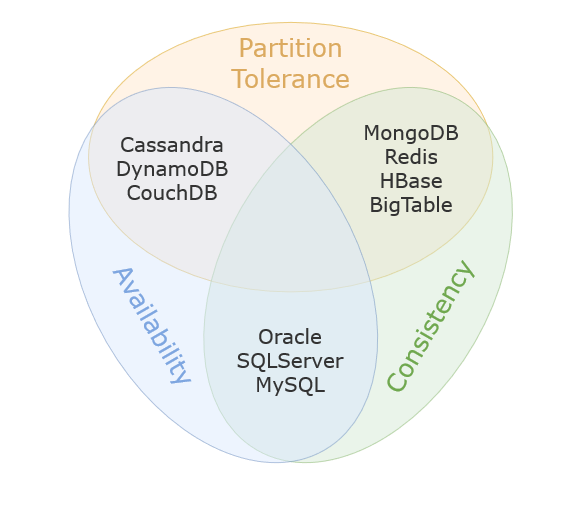
\includegraphics[height=8cm]{cap-theorem}
\end{center}
\end{figure}
\vspace{10pt} 

\noindent Mentre le soluzioni classiche (DB relazionali) garantiscono Consistenza e Disponibilità, ma hanno grossi problemi con la scalabilità orizzontale e la separazione dei dati in cluster diversi, le soluzioni NoSQL tendenzialmente garantiscono il Partizionamento, e possono quindi soddisfare soltanto una delle altre due caratteristiche.\\

\noindent In base quindi alle necessità di Ifin Sistemi, sarà necessario valutare quale tipo di database adottare anche in base al CAP theorem.

\subsection{Integrazione}
Tenendo in considerazione che lo scopo della ricerca che si è condotta rimane quello di studiare la possibilità di integrazione nello stack aziendale, è necessario valutare quanto i database individuati si prestino a tale operazione.\\

\noindent Per ognuna delle implementazioni viste precedentemente è necessario seguire regole specifiche per mettere in comunicazione il proprio applicativo con il database.\\
A volte alcune soluzioni sembrano più funzionali al proprio caso d'uso, ma non hanno un sistema ben documentato/conosciuto/sviluppato per interfacciarsi con l'applicativo che stiamo sviluppando, solitamente per motivi di compatibilità dei linguaggi e diffusione di librerie e driver utili.\\
A tale scopo elenchiamo i software individuati e le loro opzioni di integrazione, tenendo a mente che lo stack aziendale si basa sull'utilizzo di java come linguaggio di programmazione.

\subsubsection{Redis Stack}
Per quanto riguarda Redis, Redis Stack e tutti i moduli ad esso collegati, il modo più semplice e "ad alto livello" per interagire con il database è sfruttare Redis OM, costruito sulla base di Spring Data Redis. Si tratta di un modulo del progetto "Spring Data", che racchiude librerie specifiche per interagire con diversi database usando il framework Spring.

\subsubsection{Cassandra}
Cassandra può essere utilizzato in modo facile tramite Astra DB, un multi-cloud DBaaS costruito su Cassandra.
Per interagire con Astra si possono sfruttare le soluzioni più disparate, dall'utilizzo delle REST API all'implementazione di driver specifici per Java che ne facilitano l'utilizzo.

\subsubsection{MongoDB}
Mongo è una delle implementazioni NoSQL più diffuse e versatili. Si può utilizzare Atlas come "MongoDB as a Service", e anche in questo caso viene fornita la Query API per effettuare operazioni sui dati. Mongo fornisce driver per l'integrazione con Java, ma si può direttamente usare Spring Data, espressamente creato per fornire un modello familiare per datastores basato su Spring.

\subsubsection{CouchDB}
CouchDB non possiede librerie specifiche per l'integrazione e la comunicazione con applicativi scritti in Java. Quelle che esistono spesso non sono ufficiali e quindi utilizzabili "a proprio rischio e pericolo". Risulta possibile implementare la comunicazione direttamente tramite REST API, ma è dispendioso.
Esiste tuttavia una versione di CouchDB sviluppata da IBM, denominata Cloudant, che propone il servizio cloud e l'integrazione con Java.

\subsubsection{Neo4j}
Anche Neo4j ha recentemente fornito una propria piattaforma, lanciando il progetto Aura per fornire DBaaS, con supporto per integrazione con Spring Boot e Spring Data.

\subsubsection{Elasticsearch}
Elasticsearch sfrutta Elastic Cloud come soluzione distribuita.
Possiede varie funzionalità interessanti tra cui la possibilità di migrare i propri dati da un cloud all'altro, a prescindere dal provider.

\subsection{Conclusione della fase esplorativa}
Una volta studiate le opzioni esistenti sul mercato, si è passati alla fase di analisi interna per scoprire quali sono le soluzioni attualmente implementate dall'azienda, come funzionano e quali sono i loro punti critici.

%**************************************************************
\section{Panoramica su InvoiceChannel e soluzioni RDBMS adottate in Ifin Sistemi}


%**************************************************************
\section{Selezione di un'alternativa}

             % Kick-Off
% !TEX encoding = UTF-8
% !TEX TS-program = pdflatex
% !TEX root = ../tesi.tex

%**************************************************************
\chapter{Metodologie}
\label{cap:metodologie}
%**************************************************************

%\intro{Breve introduzione al capitolo}\\

%**************************************************************
\section{Strumenti e Tecnologie utilizzate}
Per poter eseguire il confronto tra le prestazioni di database relazionali e NoSQL è stato necessario preparare tutta una serie di strumenti utili a far funzionare i database stessi e al monitoraggio dei dati contenuti al loro interno.

\subsection{Docker}
Per poter effettuare test consistenti, evitare problemi di installazione e compartimentalizzare l'ambiente di lavoro, si è deciso di sfruttare Docker. Questo software permette di virtualizzare l'esecuzione di altri applicativi in ambienti chiusi e controllati, facilitando determinati processi di sviluppo. L'utilizzo di Docker in questo progetto lo rende più maneggevole e lineare.\\
Per sfruttare questo strumento è necessario installare l'engine di Docker che ci permette di gestire i vari container che andremo a creare.\\
Nello specifico, un container è una istanziazione di un'immagine, che a sua volta è uno snapshot del software che vogliamo "dockerizzare".\\
Docker ci permette di creare più container che funzionano parallelamente e indipendentemente gli uni dagli altri. Possono tuttavia comunicare utilizzando delle porte specificate nella fase di creazione dell'immagine.\\

\noindent Nel caso di questo progetto, docker risulta utile innanzitutto per gestire il funzionamento dei due DB (che saranno PostgreSQL e MongoDB), inserendoli entrambi in un rispettivo container.\\
Per facilitare poi i processi di comunicazione con i DB verranno utilizzati altri due container contenenti delle interfacce grafiche (rfispettivamente pgAdmin e MongoExpress).

\begin{figure}[htbp]
\begin{center}

\includegraphics[height=6em]{immagini/tecnologies-logos/Docker-Logo.png}
\caption{Logo di Docker}
\end{center}
\end{figure}

\subsection{PostgreSQL e tecnologie annesse}
Dopo aver scelto Docker come ambiente in cui far girare i database, alcune altre scelte legate alle tecnologie coinvolte in questa ricerca sono state prese come conseguenza.\\
Sebbene infatti sia possibile "dockerizzare" moltissimi software, agli scopi di questa tesi è risultato più comodo partire da immagini pre-esistenti ed affidabili, disponibili sulla piattaforma ufficiale del software (hub-docker).\\
Questo ha permesso di non investre troppo tempo nella preparazione degli strumenti e di concentrare le risorse disponibili nell'effettivo confronto tra database.\\

\noindent Per tutti questi motivi si è quindi scelto di usare PostgreSQL come database relazionale da portare a confronto con MongoDB.\\
PostreSQL è un database relazionale open source molto robusto che si presta bene per rappresentare le prestazioni di un generico database di questa categoria. Esso è inoltre presente nell'hub di docker con un'immagine ufficiale, ed è quindi facile da far funzionare all'interno di un container a differenza di altri prodotti simili.\\
Sebbene PostgreSQL non sia utilizzato massivamente all'interno dell'azienda, risulta comunque molto simile alle sue controparti non open source, MSSQL e Oracle Server, che sono invece largamente uaste all'interno di Ifin e sarebbero oggetto di una potenziale migrazione qualora i risultati di questa tesi si rivelassero convincenti.\\

\noindent Vale la pena di evidenziare che a differenza delle tecnologie che ricadono sotto la sigla "NoSQL", quelle legate ai database relazionali sono molto più simili tra loro, poichè condividono appunto il paradigma relazionale che sta alla base di tutte le variazioni esistenti proposte da aziende diverse in contesti diversi.\\
In questo senso, usare PostgreSQL non è una scelta incoerente con i motivi che hanno dato alla luce questo progetto.

\begin{figure}[htbp]
\begin{center}

\includegraphics[height=7em]{immagini/tecnologies-logos/postgresql-logo.png}
\caption{Logo di PostgreSQL}
\end{center}
\end{figure}

\subsection{MongoDB e tecnologie annesse}

%**************************************************************
\section{Selezione di un ambito di confronto}

%**************************************************************
\section{Modellazione del database in MongoDB}             % Concept Preview
% !TEX encoding = UTF-8
% !TEX TS-program = pdflatex
% !TEX root = ../tesi.tex

%**************************************************************
\chapter{Sperimentazione}
\label{cap:sperimentazione}
%**************************************************************
\section{Popolamento dei database}

Portata a termine la predisposizione di strumenti ed ambienti di lavoro, e determinata la struttura dei database, è ora possibile andare a caricare al loro interno i dati che li popolano.\\

\subsection{Creazione dei dati}
Per effettuare test di carico sui database è necessario che questi contengano una quantità di dati elevata. Si è scelto di generare dei dati ``fantoccio'' per automatizzare il processo.\\
Scegliendo lo strumento giusto, si possono così ottenere dati realistici in quanto a contenuto e dimensione, per fare in modo che le misurazioni effettuate sui tempi di esecuzione delle query abbiano un significato anche al di fuori dell'ambiente di test.\\
Sebbene inizialmente i dati siano stati generati tramite siti online che permettevano di esportare fino a un migliaio di tuple, è presto diventato chiaro come questo avrebbe rallentato di molto il processo di popolamento, rendendolo anche più complesso.\\

\noindent Si è quindi deciso di ricorrere ad uno strumento diverso, disponibile come pacchetto di \textit{Node.js} e installabile tramite \gls{npm} in modo da poter essere utilizzato da linea di comando.\\
Questo strumento, \textit{datamaker}, è in grado di generare un numero arbitrario di records basandosi su template forniti dall'utente. Senza contare che è molto più rapido dei sistemi online.\\
Grazie a \textit{datamaker} è stato possibile generare dei dati fittizzi secondo specifiche personalizzate, in quantità elevate.\\
Questo sistema garantisce anche un buon grado di consistenza, poiché rimane la traccia dello schema utilizzato in forma di template, cosa che invece andava spesso persa nei processi online. Anche grazie a questo è stato possibile generare dati affidabili su cui condurre i test, variando la quantità di dati presente in un file di import senza alterare in alcun modo lo schema che definisce come questi dati vengono costruiti.\\


\subsection{Formato dei dati}
Quando si parla di formato dei dati è bene specificare la differenza tra formato di importazione dei dati e formato dei dati all'interno dei database.\\
MongoDB salva i propri dati in formato \texttt{BSON}, una versione estesa del più comune \texttt{JSON}. Per la costruzione di tali dati è sufficiente creare dei file in formato \texttt{JSON}, e il database si occupa del resto.\\
Utilizzando l'interfaccia di Compass è tuttavia possibile importare i propri dati da un file in formato \texttt{CSV}. Questo può facilitare il processo, specialmente quando si è più abituati a lavorare con questo tipo di formato.\\
Per quanto riguarda PostgreSQL, anche l'interfaccia di pgAdmin permette di importare i propri dati da file, che devono essere in formato \texttt{CSV}.\\
Tale file verrà elaborato e il suo contenuto trasferito automaticamente nelle tabelle su cui si esegue questa operazione.\\

\noindent Nel caso di questo progetto, si è scelto di utilizzare file in formato \texttt{CSV} per l'importazione all'interno del database relazionale e file in formato \texttt{JSON} per l'importazione nel database NoSQL.\\
Nonostante il contenuto di documenti e tabelle sia pressochè lo stesso, proprio perchè il confronto abbia senso, la differenza sta proprio nella struttura in cui sono organizzati questi dati. Per questo motivo non sarebbe stato possibile usare lo stesso file \texttt{CSV} per popolare entrambi i database, nonostante gli strumenti utilizzati lo avrebbero permesso.\\

%**************************************************************
\section{Metodi di monitoraggio dei risultati e creazione delle query}
Per confrontare le performance delle query nei due database è necessario raccogliere dei dati sulla loro esecuzione. Nello specifico, serve sapere quanto tempo impiegano le query per essere eseguite.\\
Il tempo impiegato, tuttavia, può essere fuorviante. La notifica che per esempio riceviamo nel software pgAdmin si riferisce al tempo totale di elaborazione della richiesta, che per esempio comprende anche la latenza di connessione al network, e altri dati non relativi al tempo strettamente necessario all'esecuzione della query.\\

Per eseguire un confronto più preciso è necessario capire come estrapolare i dati che cerchiamo in entrambe le basi di dati.

\subsection{Estrapolare i tempi di esecuzione in PostgreSQL usando pgAdmin}
PostgreSQL, come molti database relazionali e non, mette a disposizione il metodo \texttt{EXPLAIN}. Quando questo viene utilizzato in testa ad una query, il risultato che si ottiene è una serie di informazioni riguardanti la sua esecuzione. Tra i vari parametri di questo metodo, quelli più interessanti per questo caso d'uso sono \texttt{ANALYZE} e \texttt{TIMING}, che possono essere specificati per ottenere informazioni specifiche riguardanti il tempo di esecuzione delle varie sezioni di query.\\
Le query che vengono eseguite in questo modo vengono comunque portate a termine dal database, anche se il risultato di eventuali operazioni di \texttt{SELECT} non viene mostrato a schermo.\\
Per impedire che questo accada è bene seguire la query con un'operazione di \textit{rollback}.\\

\noindent pgAdmin permette di utilizzare il metodo \texttt{EXPLAIN} eseguendo la query che si vuole analizzare in uno spazio apposito dell'interfaccia. Il risultato dell'operazione viene riportato in una tabella per semplificare la lettura, mentre vengono messi a disposizione anche una vista a grafo ed una tabella più complessa per il confronto tra tempi stimati dal metodo e tempi reali di esecuzione.\\
Agli scopi di questa tesi verranno prese in considerazioni le informazioni riportate nella tabella principale, dove i tempi di completamento delle operazioni sono all'occorrenza separati nei vari pezzi che compongono la query.

\subsection{Estrapolare i tempi di esecuzione in MongoDB usando Compass}
All'interno di MongoDB si utilizza un linguaggio specifico per estrapolare informazioni dai database. Se per i database relazionali si parla di Structured Query Language, in questo caso invece si usa \textit{MQL}, ovvero MongoDB Query Language, basato sulla sintassi di \textit{JavaScript}.\\

\noindent Attraverso un'ampia selezione di metodi questo linguaggio offre la possibilità di effettuare tutte le \gls{operazioni CRUD}, oltre ad alcune altre funzionalità che possono tornare utili in varie situazioni, dalla gestione dei database alla misurazione delle prestazioni delle query.\\
Utilizzando Compass, è poi possibile sfruttare una finestra apposita dell'interfaccia grafica per eseguire l'\textit{explain plan} di alcune query. Questa funzionalità è limitata tuttavia all'analisi del metodo \texttt{find()}, che corrisponde ad una select in \gls{SQL}.\\
Per gli altri metodi è necessario approfondire il funzionamento del linguaggio di MongoDB per effettuare manualmente una ricerca sui tempi di esecuzione delle varie operazioni.\\
Una volta determinato quali metodi concatenare per ottenere i risultati desiderati, è poi necessario eseguire tali comandi nella shell di MongoDB. Fortunatamente questa è accessibile sempre dall'interfaccia di Compass, rendendo il processo più lineare.\\


%**************************************************************
\section{Statistiche sulle query eseguite sui due database}
Il confronto tra i due database è stato effettuato creando sette copie di query volte ad ottenere lo stesso risultato sia sul database relazionale che su quello documentale. Il risultato di questo tipo di analisi evidenzia come le diverse strutture di archiviazione dei dati e le diverse architetture all'interno dei database possono garantire risultati migliori o peggiori in base ai casi d'uso.\\
La creazione delle query è stata basata su una esemplificazione dei casi d'uso più comuni individuati per InvoicheChannel.

\subsection{Query 1}
La prima query è piuttosto semplice. Effettua una ricerca generica per elencare tutte le invoice e le operations ad esse collegate.\\

\begin{figure}[htbp]
\begin{center}
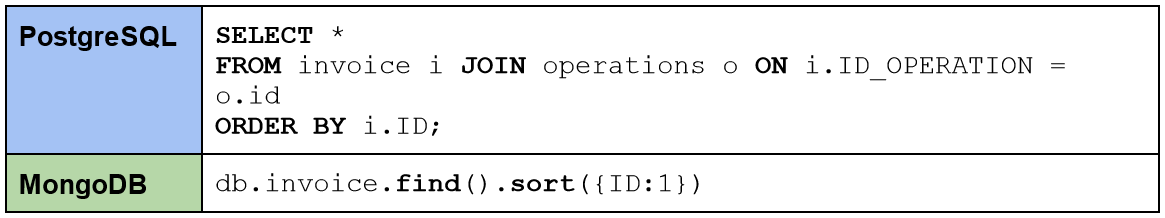
\includegraphics[height=7em]{immagini/query/query1.png}
\caption{Codice della query numero 1, scritto in entrambi i linguaggi}
\end{center}
\end{figure}

\noindent Nota: PostgreSQL crea automaticamente gli indici sulle primary keys, quindi sono stati indicizzati anche i campi ID dei documenti in MongoDB. Questo è stato fatto per effettuare un confronto alla pari, ma è anche dovuto al fatto che intorno ai 200.000 documenti MongoDB non permette più di effettuare operazioni di \texttt{sort()} se non viene integrato l'uso di indici.\\

\noindent Nella seguente tabella possiamo vedere i risultati del confronto sui tempi ottenuti ripetendo la stessa query su database popolati con un numero sempre maggiore di elementi.\\

\begin{figure}[htbp]
\begin{center}
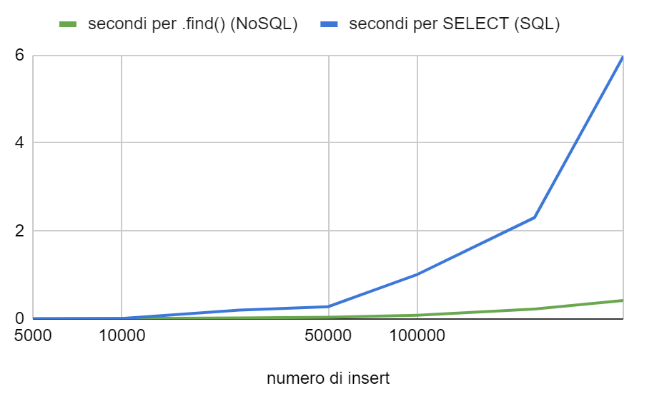
\includegraphics[height=20em]{immagini/query/query1_results.png}
\caption{Risultato del confronto, query numero 1}
\end{center}
\end{figure}

\noindent Dal grafico si evince quanto già scoperto durante lo studio delle tecnologie coinvolte nel confronto. L'utilizzo di documenti incorporati (in questo caso i dati dell'operation che riguarda l'invoice sono contenuti nel documento dell'invoice stessa) permette a MongoDB di evitare le operazioni di \texttt{join}, che rallentano di molto l'esecuzione delle query in PostgreSQL.\\

\noindent Possiamo notare come la differenza sia ancora più evidente se cerchiamo gli stessi dati applicando una condizione di ricerca.\\

%--------------------------------------------------------------

\subsection{Query 2}
Cerchiamo tutte le invoice e le operations associate, questa volta limitandoci alle sole fatture che soddisfano una specifica condizione sul proprio numero identificativo.\\

\begin{figure}[htbp]
\begin{center}
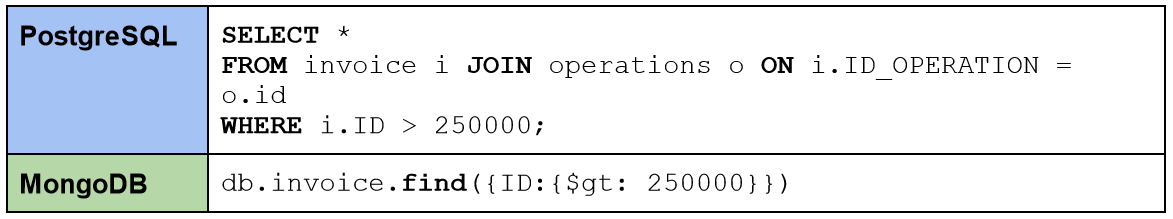
\includegraphics[height=7em]{immagini/query/query2.png}
\caption{Codice della query numero 2, scritto in entrambi i linguaggi}
\end{center}
\end{figure}

\noindent In questo caso PostgreSQL farà uso di indici per andare a scorrere invoice e verificare le condizioni che validano i dati. Introduciamo quindi l'indice su \texttt{ID} anche per il database di MongoDB.\\

\begin{figure}[htbp]
\begin{center}
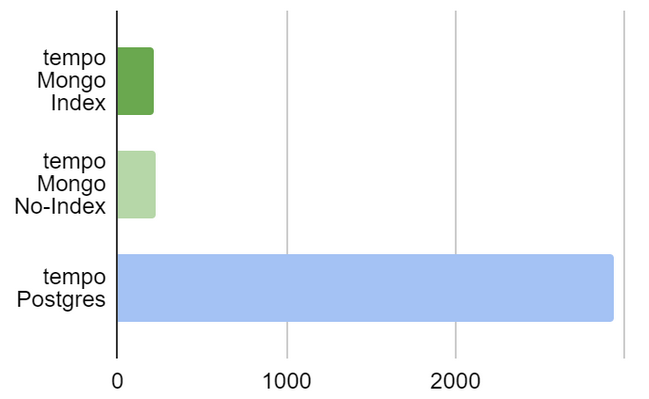
\includegraphics[height=16em]{immagini/query/query2_results1.png}
\caption{Risultato del confronto, query numero 2}
\end{center}
\end{figure}

\noindent Questa query è stata testata su database contenenti 500.000 elementi, chiedendo loro di restituirne soltanto la metà.\\
Si può vedere come, a prescindere dalla presenza dell'indice, MongoDB sia comunque più veloce di un ordine di grandezza.\\
Inoltre, grazie agli strumenti messi a disposizione da PostgreSQL, possiamo anche vedere come è stato speso il tempo all'interno di questa query:

\begin{figure}[htbp]
\begin{center}
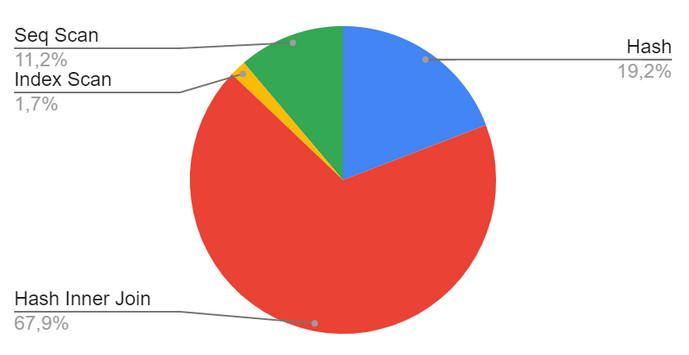
\includegraphics[height=15em]{immagini/query/query2_results2.png}
\caption{Utilizzo del tempo di esecuzione, query numero 2}
\end{center}
\end{figure}

\noindent Quasi il 70\% del tempo è dedicato all'operazione di \texttt{join}, di cui invece MongoDB non si deve preoccupare (in questo caso).\\
La sola operazione di Index Scan occupa PostgreSQL per circa 90 ms, un tempo che sarebbe estremamente competitivo.\\

%--------------------------------------------------------------

\subsection{Query 3}
A confermare la tesi portata con la seconda query, effettuare una ricerca su un campo non indicizzato, in cui non è richiesto alcuna operazione di \texttt{join}, produce risultati più o meno simili per entrambi i sistemi: ~240ms per MongoDB contro i ~300ms per Postgres.\\
Anche in questo caso i test sono stati effettuati su database contenenti 500.000 elementi. Non sono riportati grafici a causa della minima differenza di prestazioni.\\

\begin{figure}[htbp]
\begin{center}
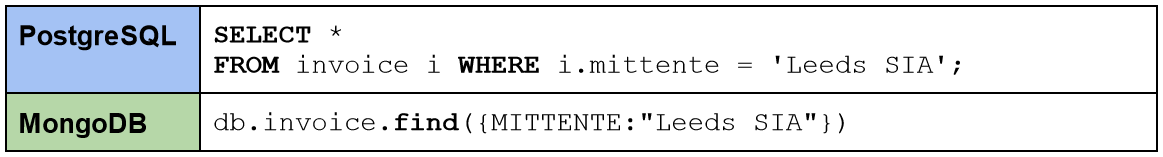
\includegraphics[height=5em]{immagini/query/query3.png}
\caption{Codice della query numero 3, scritto in entrambi i linguaggi}
\end{center}
\end{figure}

%--------------------------------------------------------------

\subsection{Query 4}
Questa query cerca di evidenziare un'altra differenza importante tra i due database, dovuta al diverso metodo di archiviazione dei dati (documenti \texttt{JSON} o tabelle).\\

\begin{figure}[htbp]
\begin{center}
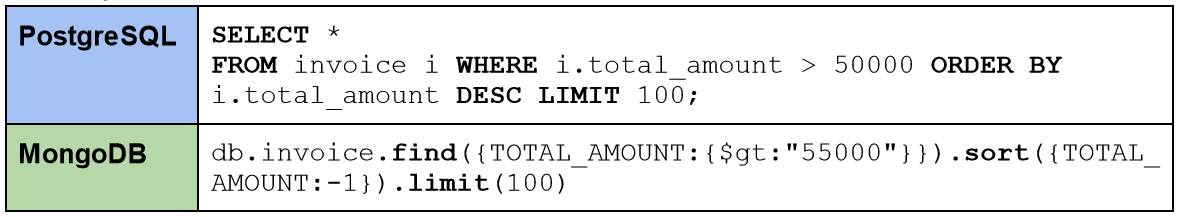
\includegraphics[height=7em]{immagini/query/query4.png}
\caption{Codice della query numero 4, scritto in entrambi i linguaggi}
\end{center}
\end{figure}

\noindent In questo caso vengono testati entrambi i database con 100.000 elementi inseriti.\\
Si vogliono trovare i documenti con data di invio più recente. Dover accedere al contenuto dei campi sembrerebbe essere un lavoro più dispendioso quando si tratta di un campo di un documento, piuttosto che un campo di una tabella. Si nota infatti che il risultato ottenuto conferma questa tesi.\\

\begin{figure}[htbp]
\begin{center}
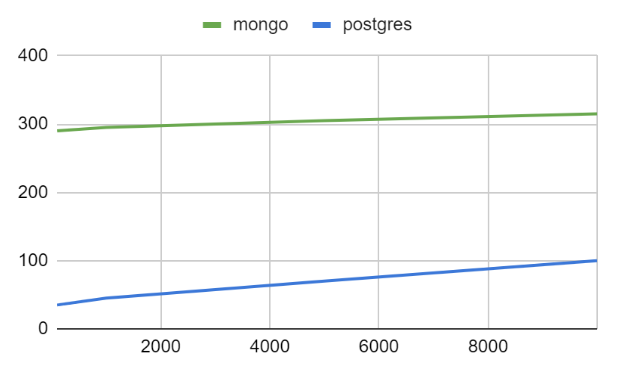
\includegraphics[height=15em]{immagini/query/query4_results.png}
\caption{Risultato del confronto, query numero 4}
\end{center}
\end{figure}

%--------------------------------------------------------------

\subsection{Query 5}
Viene testata ora una query più complessa, utilizzata per effettuare l'update di determinati campi all'interno del database. Nello specifico, si vogliono simulare l'update della causale della fattura, con delle condizioni che comprendono dati dell'operation ad essa collegata.\\

\begin{figure}[htbp]
\begin{center}
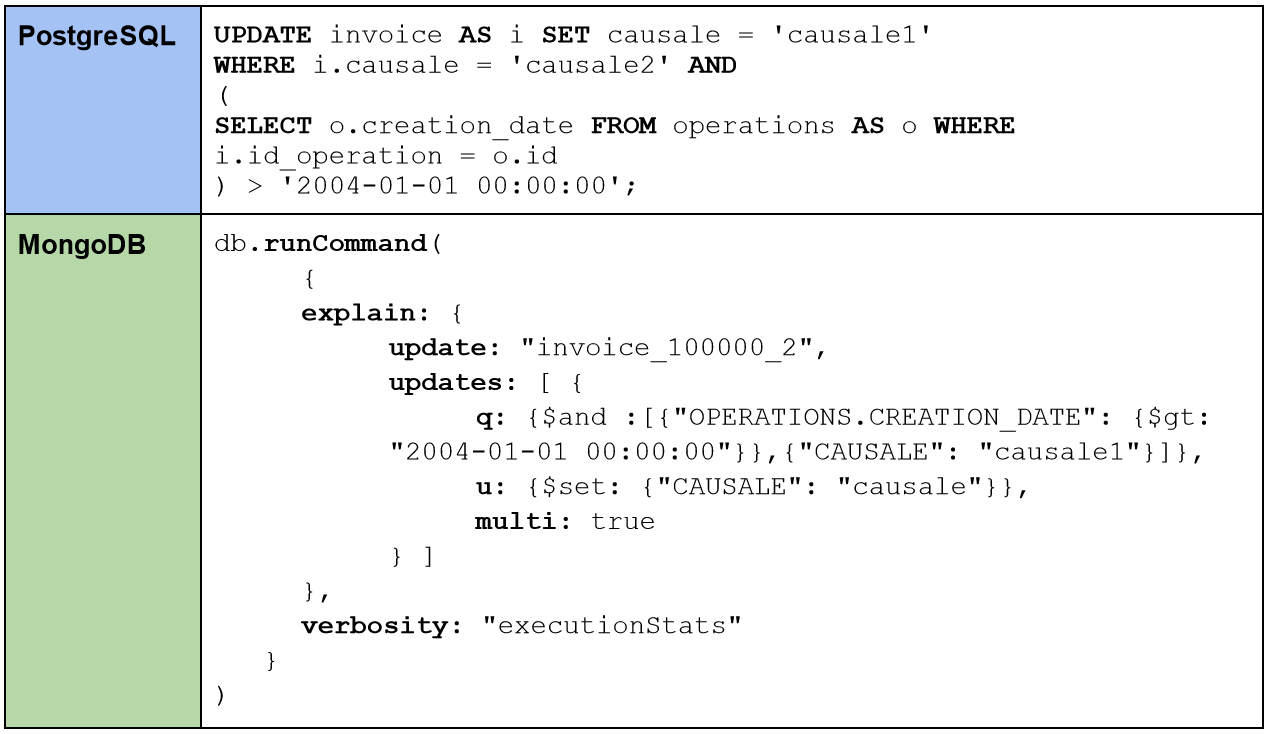
\includegraphics[height=20em]{immagini/query/query5.png}
\caption{Codice della query numero 5, scritto in entrambi i linguaggi}
\end{center}
\end{figure}

\noindent Per eseguire questa query in mongo la concatenazione dei metodi è più complessa, come si può notare dall'immagine che riporta il codice.\\
Purtroppo Compass mette a disposizione l'interfaccia explain solo per il metodo \texttt{find()}. Come detto in precedenza dobbiamo quindi passare tramite \textit{mongosh}, il terminale di MongoDB su cui si possono eseguire tutti i comandi nella sua sintassi specifica.\\
Inoltre, il sistema utilizzato precedentemente (ovvero concatenare il metodo \texttt{explain()} a fine query) non è disponibile per l'operazione di update, e bisogna quindi usare una sintassi più completa che prevede l'uso del metodo \texttt{runCommand()}, visibile in tabella.\\

\noindent Nuovamente, il grafico non viene riportato poiché lineare. L'unico dato utile che traspare è la costante differenza nei tempi di esecuzione, che anche in questo caso favoriscono MongoDB, aggirandosi intorno ai 105 ms. Per postgres abbiamo tempi all'incirca doppi.\\

%--------------------------------------------------------------

\subsection{Query 6}
Questa query è simile alla precedente. In questo caso tuttavia l'aggiornamento viene fatto sulla tabella \texttt{OPERATIONS}, e la condizione risiede in tabella \texttt{INVOICE}.\\

\begin{figure}[htbp]
\begin{center}
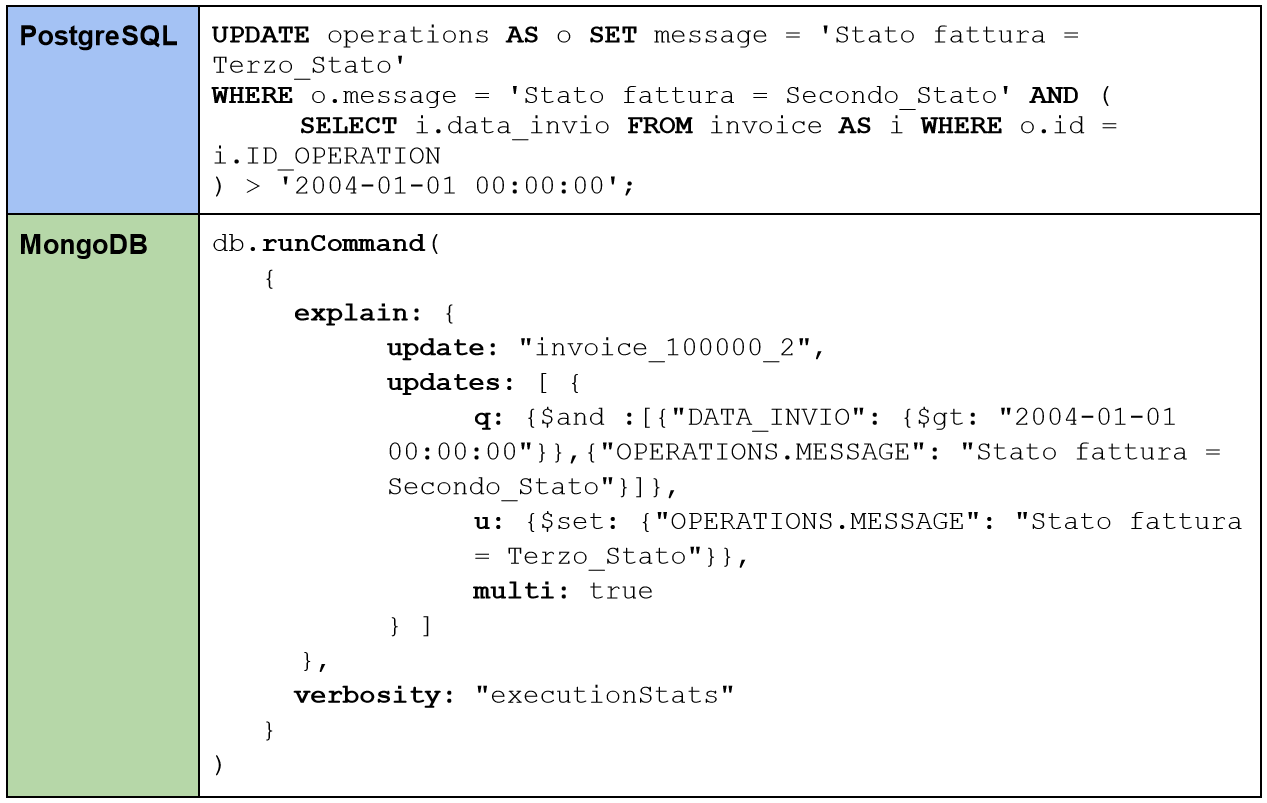
\includegraphics[height=22em]{immagini/query/query6.png}
\caption{Codice della query numero 6, scritto in entrambi i linguaggi}
\end{center}
\end{figure}

\noindent La query su PostgreSQL impiega dai 2 ai 5 minuti per essere portata a termine su un database contenente 100.000 elementi.\\
Possiamo notare come quasi tutto questo tempo sia utilizzato per effettuare uno scan della tabella \texttt{OPERATIONS}, che viene poi aggiornata.\\

\begin{figure}[htbp]
\begin{center}
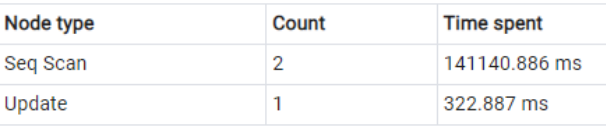
\includegraphics[height=5em]{immagini/query/query6_results.png}
\caption{Suddivisione dei tempi di esecuzione per la query numero 6 in PostgreSQL}
\end{center}
\end{figure}

\noindent MongoDB impiega soltanto 65 millisecondi per effettuare tutte le operazioni.\\
Ripetendo la query su database più ampi il risultato non cambia. Per 250.000 elementi PostgreSQL impiega più di trenta minuti, MongoDB si mantiene sotto i 200 millisecondi. Il tempo raddoppia quando all'interno del database sono contenuti 500.000 elementi. Per questa quantità di dati, PostgreSQL non restituisce un risultato in tempi utili.\\

%--------------------------------------------------------------

\subsection{Query 7}
Quest'ultima query rappresenta un altro caso d'uso importante.

\begin{figure}[htbp]
\begin{center}
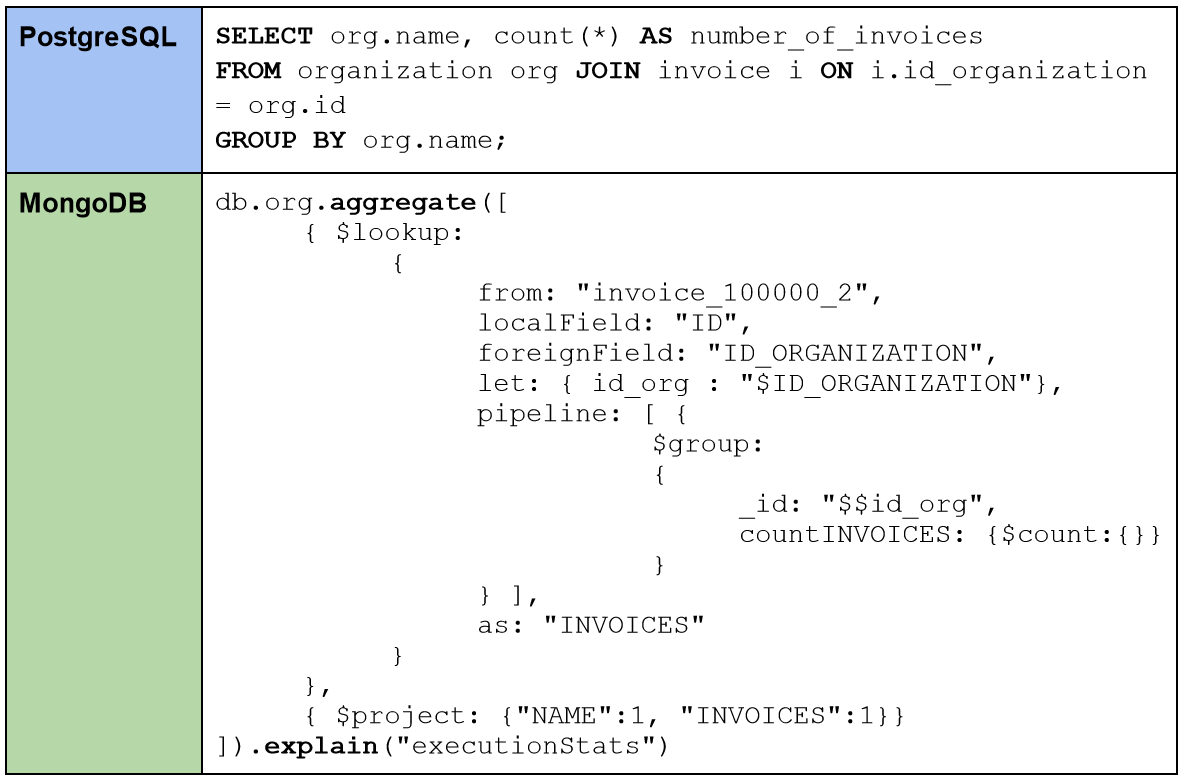
\includegraphics[height=22em]{immagini/query/query7.png}
\caption{Codice della query numero 7, scritto in entrambi i linguaggi}
\end{center}
\end{figure}

\noindent Come già menzionato, MongoDB è sì un database NoSQL, ma tecnicamente è considerabile anche ``relazionale'', perchè consente di effettuare operazioni di \textit{lookup} tra \textit{collection} diverse per unire informazioni altrimenti separate. Questa, tuttavia, non è sicuramente la feature di punta di un database documentale, e si traduce quindi in un'operazione piuttosto lenta rispetto ad altre operazioni per cui un un database di questo tipo è stato espressamente studiato.\\

\noindent Tutto questo è dimostrato dai dati statistici raccolti durante l'esecuzione delle query.\\
Per PostgreSQL si tratta di una join piuttosto semplice, accoppiata ad un raggruppamento. Il tempo di esecuzione si aggira intorno ai 65 ms se le tabelle \texttt{INVOICE} e \texttt{ORGANIZATION} contengono 100.000 elementi ciascuna.\\
MongoDB impiega tra i 5 e i 6 secondi per la stessa operazione, con la stessa quantità di dati.

\begin{figure}[htbp]
\begin{center}
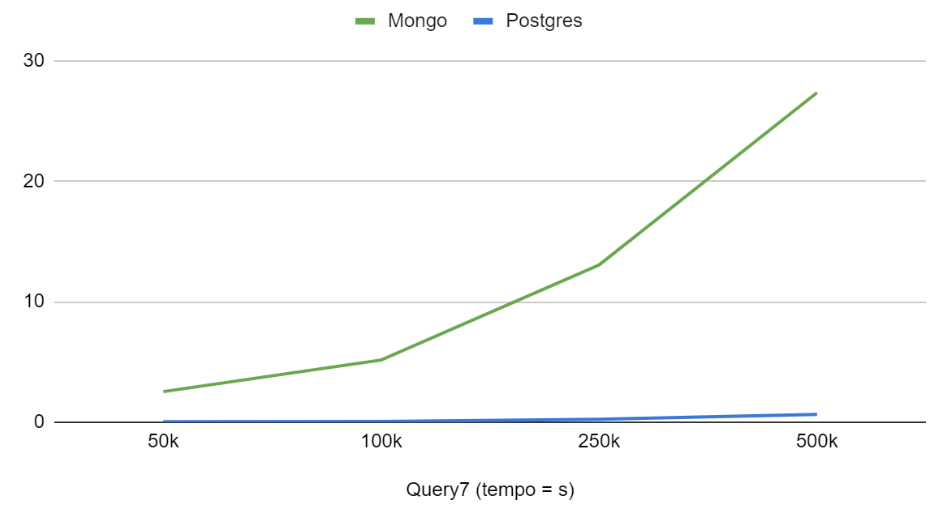
\includegraphics[height=15em]{immagini/query/query7_results.png}
\caption{Risultato del confronto, query numero 7}
\end{center}
\end{figure}

\noindent Con questa query si conclude la fase di confronto diretto tra i tempi di esecuzione delle operazioni sui due database.Vale la pena di evidenziare un fattore che sicuramente salta all'occhio leggendo le precedenti pagine: la complessità del linguaggio utilizzato per le query di MongoDB non è trascurabile e rispetto all'immediatezza di \gls{SQL} risulta piuttosto impegnativo da imparare, utilizzare e comprendere.

%**************************************************************
\section{Inserimento della fattura integrale}
\label{sec:fattura-integrale}
Uno dei casi d'uso di interesse per l'analisi condotta su InvoiceChannel è quello che riguarda il salvataggio delle fatture.\\
Sebbene parte dei dati che le compongono sia salvata nella tabella invoice, per velocizzare l'accesso alle informazioni più importanti la fattura viene anche salvata per intero in formato \texttt{XML}.\\

\noindent Questo ovviamente non può essere fatto all'interno del database, principalmente perchè salvare dei dati così grandi all'interno di un unico campo non è desiderabile.\\
All'estremo opposto c'è la possibilità di elaborare il contenuto del file per scomporlo in campi salvabili e indicizzabili, potendo così ricomporre la fattura quando necessario. Anche questa soluzione ha dei problemi, perchè effettuare operazioni di questo tipo su ogni fattura introdotta nel sistema creerebbe probabilmente un collo di bottiglia, e anche ricomporla quando necessario potrebbe rivelarsi costoso o non pratico.\\

\noindent La soluzione, come spesso succede, sta nel mezzo, e se ne trova un esempio all'interno dell'architettura di MongoDB.\\
Come è stato visto, MongoDB salva i propri documenti in formato \texttt{JSON}, introducendo degli ``effetti collaterali'' che tornano utili al nostro caso d'uso.\\
L'idea è di convertire le fatture da \texttt{XML} a \texttt{JSON} per poi salvarle integralmente all'interno di una collection apposita.\\
In questo modo la fattura sarebbe sempre a disposizione per intero all'interno del database, come se fosse stato inserito il file \texttt{XML} in un campo di tabella. Allo stesso tempo sarebbe facile effettuare ricerche sui ``campi'' che compongono la fattura, per natura stessa dei file \texttt{JSON}, senza dover fare alcuna operazione di scomposizione e ricostruzione del file, se non per l'iniziale traduzione da un formato all'altro.\\

\noindent Tale trasformazione è bidirezionale, quindi così come si è passati dall'\texttt{XML} al \texttt{JSON} si può fare il contrario senza alcuna perdita di dati. Questo è importante perchè a livello legale \texttt{XML} rimane il formato ufficiale per le fatture elettroniche, quindi in caso di necessità si può ricostruire l'originale.\\

\noindent Tutto questo ovviamente ha un costo, e sta a chi crea un sistema di questo tipo il compito di soppesare pro e contro. MongoDB supporta l'inserimento di file \texttt{BSON} fino a 16 MB e una fattura tradotta in formato \texttt{JSON} occupa circa 5 KB, quindi sebbene appaia come un file ``grande'' all'occhio umano, si tratta di una dimensione bel al di sotto dei limiti strutturali del database. Le prestazioni non sarebbero intaccate da questo tipo di soluzione, anche quando si considera l'archiviazione di centinaia di migliaia di fatture, specialmente se si fa uso di indici.\\
Anche il costo della traduzione da \texttt{XML} a \texttt{JSON} va sicuramente rendicontato, ma dai test condotti non sembra avere un grosso impatto. Utilizzando uno strumento esterno basato su \gls{npm} (come \textit{datamaker}) è possibile automatizzare questo processo ad un bassissimo costo computazionale.\\


             % Product Prototype
% !TEX encoding = UTF-8
% !TEX TS-program = pdflatex
% !TEX root = ../tesi.tex

%**************************************************************
\chapter{Sperimentazione}
\label{cap:sperimentazione}
%**************************************************************
\section{Popolamento dei database}

Portata a termine la predisposizione di strumenti ed ambienti di lavoro, e determinata la struttura dei database, è ora possibile andare a caricare al loro interno i dati che li popolano.\\

\subsection{Creazione dei dati}
Per effettuare test di carico sui database è necessario che questi contengano una quantità di dati elevata. Si è scelto di generare dei dati ``fantoccio'' per automatizzare il processo.\\
Scegliendo lo strumento giusto, si possono così ottenere dati realistici in quanto a contenuto e dimensione, per fare in modo che le misurazioni effettuate sui tempi di esecuzione delle query abbiano un significato anche al di fuori dell'ambiente di test.\\
Sebbene inizialmente i dati siano stati generati tramite siti online che permettono di esportare fino a un migliaio di tuple, è presto diventato chiaro come questo avrebbe rallentato di molto il processo di popolamento, rendendolo anche più complesso.\\

\noindent Si è quindi deciso di ricorrere ad uno strumento diverso, disponibile come pacchetto di \textit{Node.js} e installabile tramite \gls{npm}\ped{G} (\textit{node package manager}) in modo da poter essere utilizzato da linea di comando.\\
Questo strumento, \textit{datamaker}\cite{site:datamaker}, è in grado di generare un numero arbitrario di records basandosi su template forniti dall'utente. Senza contare che è molto più rapido dei sistemi online.\\
Grazie a \textit{datamaker} è stato possibile generare dei dati fittizzi secondo specifiche personalizzate, in quantità elevate.\\
Questo sistema garantisce anche un buon grado di consistenza, poiché rimane la traccia dello schema utilizzato in forma di template, cosa che invece andava spesso persa nei processi online. Anche grazie a questo è stato possibile generare dati affidabili su cui condurre i test, variando la quantità di dati presente in un file di import senza alterare in alcun modo lo schema che definisce come questi dati vengono costruiti.\\


\subsection{Formato dei dati}
Quando si parla di formato dei dati è bene specificare la differenza tra formato di importazione dei dati e formato dei dati all'interno dei database.\\
MongoDB salva i propri dati in formato \texttt{BSON}, una versione estesa del più comune \texttt{JSON}. Per la costruzione di tali dati è sufficiente creare dei file in formato \texttt{JSON}, e il database si occupa del resto.\\
Utilizzando l'interfaccia di Compass è tuttavia possibile importare i propri dati da un file in formato \texttt{CSV}. Questo può facilitare il processo, specialmente quando si è più abituati a lavorare con questo tipo di formato.\\
Per quanto riguarda PostgreSQL, anche l'interfaccia di pgAdmin permette di importare i propri dati da file, che devono essere in formato \texttt{CSV}.\\
Tale file verrà elaborato e il suo contenuto trasferito automaticamente nelle tabelle su cui si esegue questa operazione.\\

\noindent Nel caso di questo progetto, si è scelto di utilizzare file in formato \texttt{CSV} per l'importazione all'interno del database relazionale e file in formato \texttt{JSON} per l'importazione nel database NoSQL.\\
Nonostante il contenuto di documenti e tabelle sia pressochè lo stesso, proprio perchè il confronto abbia senso, la differenza sta proprio nella struttura in cui sono organizzati questi dati. Per questo motivo non sarebbe stato possibile usare lo stesso file \texttt{CSV} per popolare entrambi i database, nonostante gli strumenti utilizzati lo avrebbero permesso.\\

%**************************************************************
\section{Metodi di monitoraggio dei risultati e creazione delle query}
Per confrontare le performance delle query nei due database è necessario raccogliere dei dati sulla loro esecuzione. Nello specifico, serve sapere quanto tempo impiegano le query per essere eseguite.\\
Il tempo impiegato, tuttavia, può essere fuorviante. La notifica che per esempio riceviamo nel software pgAdmin si riferisce al tempo totale di elaborazione della richiesta, che per esempio comprende anche la latenza di connessione al network, e altri dati non relativi al tempo strettamente necessario all'esecuzione della query.\\

Per eseguire un confronto più preciso è necessario capire come estrapolare i dati che cerchiamo in entrambe le basi di dati.

\subsection{Estrapolare i tempi di esecuzione in PostgreSQL usando pgAdmin}
PostgreSQL, come molti database relazionali e non, mette a disposizione il metodo \texttt{EXPLAIN}\cite{site:postgresdocs}. Quando questo viene utilizzato in testa ad una query, il risultato che si ottiene è una serie di informazioni riguardanti la sua esecuzione. Tra i vari parametri di questo metodo, quelli più interessanti per questo caso d'uso sono \texttt{ANALYZE} e \texttt{TIMING}, che possono essere specificati per ottenere informazioni specifiche riguardanti il tempo di esecuzione delle varie sezioni di query.\\
Le query che vengono eseguite in questo modo vengono comunque portate a termine dal database, anche se il risultato di eventuali operazioni di \texttt{SELECT} non viene mostrato a schermo.\\
Per impedire che questo accada è bene seguire la query con un'operazione di \textit{rollback}.\\

\noindent pgAdmin permette di utilizzare il metodo \texttt{EXPLAIN} eseguendo la query che si vuole analizzare in uno spazio apposito dell'interfaccia\cite{site:pgAdmin}. Il risultato dell'operazione viene riportato in una tabella per semplificare la lettura, mentre vengono messi a disposizione anche una vista a grafo ed una tabella più complessa per il confronto tra tempi stimati dal metodo e tempi reali di esecuzione.\\
Agli scopi di questa tesi, verranno prese in considerazione le informazioni riportate nella tabella principale, dove i tempi di completamento delle operazioni sono all'occorrenza separati nei vari pezzi che compongono la query.

\subsection{Estrapolare i tempi di esecuzione in MongoDB usando Compass}
All'interno di MongoDB si utilizza un linguaggio specifico per estrapolare informazioni dai database\cite{site:mongodb}. Se per i database relazionali si parla di Structured Query Language, in questo caso invece si usa \textit{MQL}, ovvero MongoDB Query Language, basato sulla sintassi di \textit{JavaScript}.\\

\noindent Attraverso un'ampia selezione di metodi questo linguaggio offre la possibilità di effettuare tutte le \gls{operazioni CRUD}\ped{G}, oltre ad alcune altre funzionalità che possono tornare utili in varie situazioni, dalla gestione dei database alla misurazione delle prestazioni delle query.\\
Utilizzando Compass, è poi possibile sfruttare una finestra apposita dell'interfaccia grafica per eseguire l'\textit{explain plan} di alcune query\cite{site:mongodbcompass}. Questa funzionalità è limitata tuttavia all'analisi del metodo \texttt{find()}, che corrisponde ad una select in \gls{SQL}\ped{G}.\\
Per gli altri metodi è necessario approfondire il funzionamento del linguaggio di MongoDB per effettuare manualmente una ricerca sui tempi di esecuzione delle varie operazioni.\\
Una volta determinato quali metodi concatenare per ottenere i risultati desiderati, è poi necessario eseguire tali comandi nella shell di MongoDB. Fortunatamente questa è accessibile sempre dall'interfaccia di Compass, rendendo il processo più lineare.\\


%**************************************************************
\section{Statistiche sulle query eseguite sui due database}
Il confronto tra i due database è stato effettuato creando sette copie di query volte ad ottenere lo stesso risultato sia sul database relazionale che su quello documentale. Il risultato di questo tipo di analisi evidenzia come le diverse strutture di archiviazione dei dati e le diverse architetture all'interno dei database possono garantire risultati migliori o peggiori in base ai casi d'uso.\\
La creazione delle query è stata basata su una esemplificazione dei casi d'uso più comuni individuati per InvoicheChannel.

\subsection{Query 1}
La prima query, esposta in \autoref{fig:query1}, è piuttosto semplice. Effettua una ricerca generica per elencare tutte le invoice e le operations ad esse collegate.\\

\begin{figure}[htbp]
\begin{center}
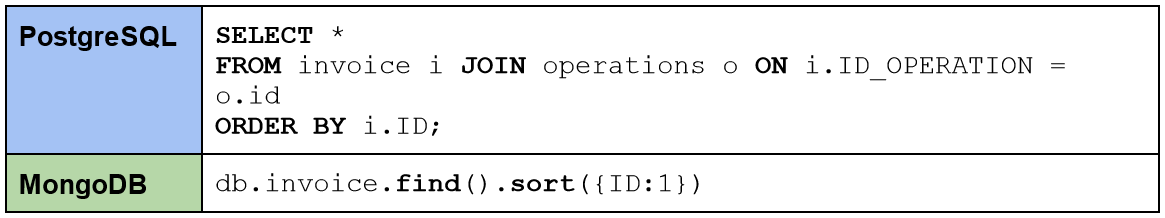
\includegraphics[height=7em]{immagini/query/query1.png}
\caption{Codice della query numero 1, scritto in entrambi i linguaggi}
\label{fig:query1}
\end{center}
\end{figure}

\noindent Facciamo notare che PostgreSQL crea automaticamente gli indici sulle primary keys, quindi sono stati indicizzati anche i campi ID dei documenti in MongoDB. Questo è stato fatto per effettuare un confronto alla pari, ma è anche dovuto al fatto che intorno ai 200.000 documenti MongoDB non permette più di effettuare operazioni di \texttt{sort()} se non viene integrato l'uso di indici.\\
\noindent Nella \autoref{tab:query1} possiamo vedere i risultati del confronto sui tempi ottenuti ripetendo la stessa query su database popolati con un numero sempre maggiore di elementi.\\

\begin{table}
\begin{center}
    \renewcommand{\arraystretch}{1.5}
    
    \centering
    \begin{longtable}{| C{2.5cm} | C{4cm} | C{4cm} |}
        
        \hline
        \rowcolor{mongogreen}
        \textbf{Numero di elementi} & \textbf{Secondi impiegati: PostgreSQL} & \textbf{Secondi impiegati: MongoDB} \\
        
        \hline
        5000 & 0,0047 & 0,007 \\
        \hline 
        10000 & 0,0111 & 0,014 \\
        \hline 
        25000 & 0,0253 & 0,2039 \\
        \hline 
        50000 & 0,0423 & 0,2793 \\
        \hline 
        100000 & 0,0833 & 1,0081 \\
        \hline 
        250000 & 0,2277 & 2,3048 \\
        \hline
        500000 & 0,4204 & 5,9701 \\
        \hline
        
        \caption{Confronto sui tempi di esecuzione della query numero 1}
        \label{tab:query1}
    \end{longtable}
\end{center}
\end{table}

\noindent Dal grafico in \autoref{fig:query1.2} si evince quanto già scoperto durante lo studio delle tecnologie coinvolte nel confronto. L'utilizzo di documenti incorporati (in questo caso i dati dell'operation che riguarda l'invoice sono contenuti nel documento dell'invoice stessa) permette a MongoDB di evitare le operazioni di \texttt{join}, che rallentano di molto l'esecuzione delle query in PostgreSQL.\\

\begin{figure}[htbp]
\begin{center}
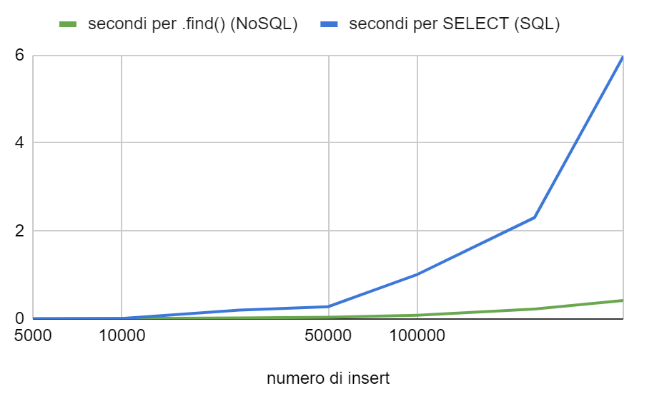
\includegraphics[height=20em]{immagini/query/query1_results.png}
\caption{Risultato del confronto, query numero 1}
\label{fig:query1.2}
\end{center}
\end{figure}

\noindent Possiamo notare come la differenza sia ancora più evidente se cerchiamo gli stessi dati applicando una condizione di ricerca.\\

%--------------------------------------------------------------

\subsection{Query 2}
Con la seconda query, esposta in \autoref{fig:query2}, cerchiamo tutte le invoice e le operations ad esse associate, questa volta limitandoci alle sole fatture che soddisfano una specifica condizione sul proprio numero identificativo.\\

\begin{figure}[htbp]
\begin{center}
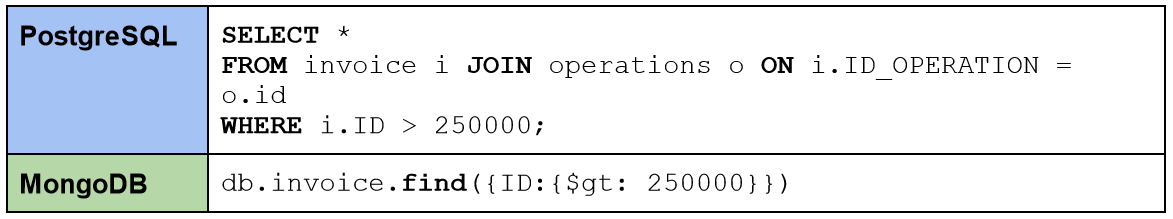
\includegraphics[height=7em]{immagini/query/query2.png}
\caption{Codice della query numero 2, scritto in entrambi i linguaggi}
\label{fig:query2}
\end{center}
\end{figure}

\noindent In questo caso PostgreSQL farà uso di indici per andare a scorrere invoice e verificare le condizioni che validano i dati. Introduciamo quindi l'indice su \texttt{ID} anche per il database di MongoDB.\\

\begin{figure}[htbp]
\begin{center}
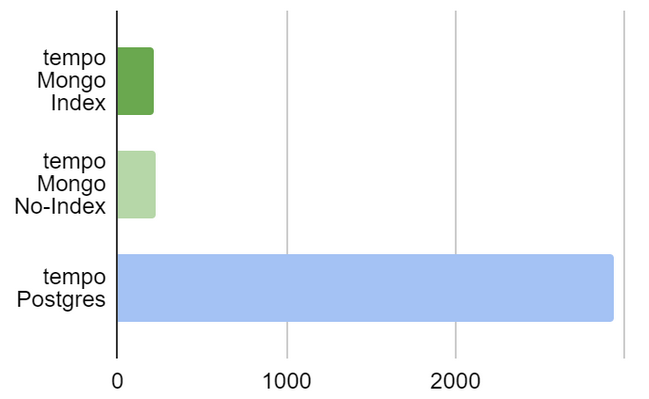
\includegraphics[height=16em]{immagini/query/query2_results1.png}
\caption{Risultato del confronto, query numero 2}
\label{fig:query2.2}
\end{center}
\end{figure}

\noindent Questa query è stata testata su database contenenti 500.000 elementi, chiedendo loro di restituirne soltanto la metà.\\
In \autoref{fig:query2.2} si può vedere come, a prescindere dalla presenza dell'indice, MongoDB sia comunque più veloce di un ordine di grandezza.\\
Inoltre, grazie agli strumenti messi a disposizione da PostgreSQL, possiamo anche vedere come è stato speso il tempo all'interno di questa query (\autoref{fig:query2.3}).

\begin{figure}[htbp]
\begin{center}
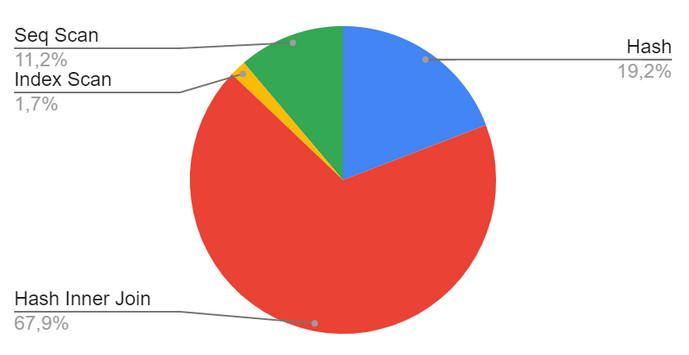
\includegraphics[height=15em]{immagini/query/query2_results2.png}
\caption{Utilizzo del tempo di esecuzione, query numero 2}
\label{fig:query2.3}
\end{center}
\end{figure}

\noindent Quasi il 70\% del tempo è dedicato all'operazione di \texttt{join}, di cui invece MongoDB non si deve preoccupare (in questo caso).\\
La sola operazione di Index Scan occupa PostgreSQL per circa 90 ms, un tempo che sarebbe estremamente competitivo.\\

%--------------------------------------------------------------

\subsection{Query 3}
A confermare la tesi portata con la seconda query, effettuare una ricerca su un campo non indicizzato, in cui non è richiesto alcuna operazione di \texttt{join}, produce risultati più o meno simili per entrambi i sistemi: ~240ms per MongoDB contro i ~300ms per Postgres (query esposta in \autoref{fig:query3}).\\
Anche in questo caso i test sono stati effettuati su database contenenti 500.000 elementi. Non sono riportati grafici a causa della minima differenza di prestazioni.\\

\begin{figure}[htbp]
\begin{center}
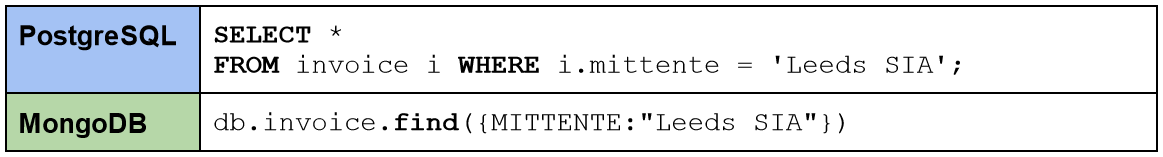
\includegraphics[height=5em]{immagini/query/query3.png}
\caption{Codice della query numero 3, scritto in entrambi i linguaggi}
\label{fig:query3}
\end{center}
\end{figure}

%--------------------------------------------------------------

\subsection{Query 4}
La query esposta in \autoref{fig:query4} risulta utile per evidenziare un'altra differenza importante tra i due database, dovuta al diverso metodo di archiviazione dei dati (documenti \texttt{JSON} o tabelle).\\

\begin{figure}[htbp]
\begin{center}
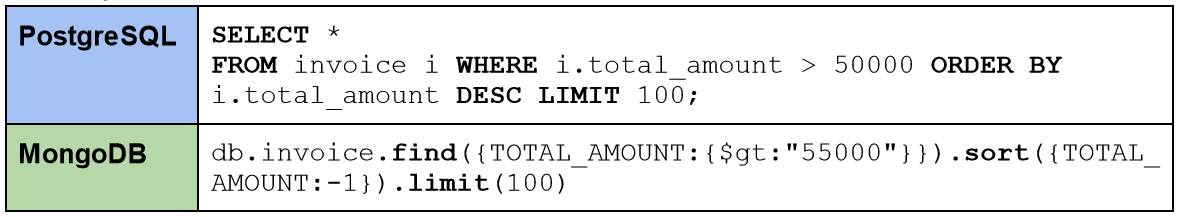
\includegraphics[height=7em]{immagini/query/query4.png}
\caption{Codice della query numero 4, scritto in entrambi i linguaggi}
\label{fig:query4}
\end{center}
\end{figure}

\noindent In questo caso vengono testati entrambi i database con 100.000 elementi inseriti.\\
Si vogliono trovare i documenti con data di invio più recente. Dover accedere al contenuto dei campi sembrerebbe essere un lavoro più dispendioso quando si tratta di un campo di un documento, piuttosto che un campo di una tabella. Nel grafico riportato in \autoref{fig:query4.2} si nota infatti che il risultato ottenuto conferma questa tesi.\\

\begin{figure}[htbp]
\begin{center}
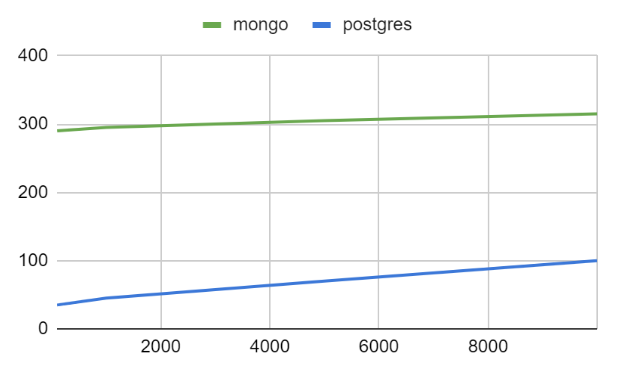
\includegraphics[height=15em]{immagini/query/query4_results.png}
\caption{Risultato del confronto, query numero 4}
\label{fig:query4.2}
\end{center}
\end{figure}

%--------------------------------------------------------------

\subsection{Query 5}
Viene testata ora una query più complessa, utilizzata per effettuare l'update di determinati campi all'interno del database. Nello specifico, si vogliono simulare l'update della causale della fattura, con delle condizioni che comprendono dati dell'operation ad essa collegata.\\

\begin{figure}[htbp]
\begin{center}
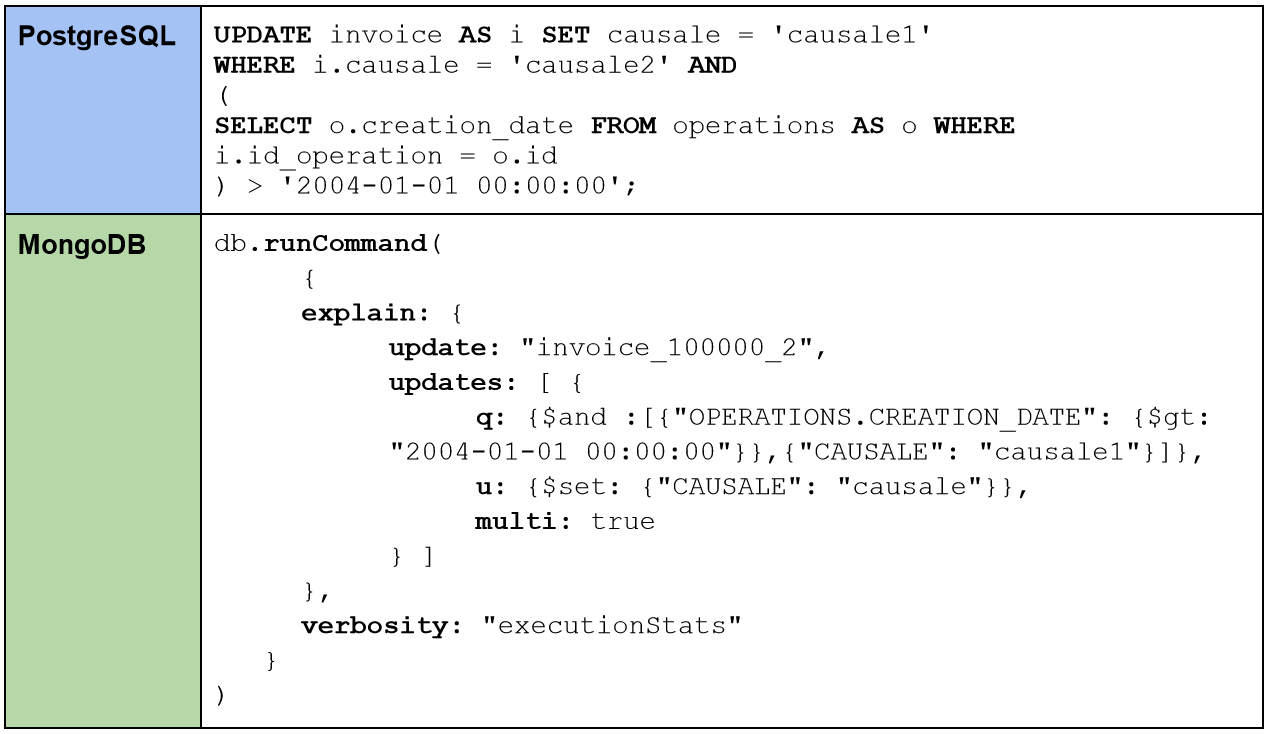
\includegraphics[height=20em]{immagini/query/query5.png}
\caption{Codice della query numero 5, scritto in entrambi i linguaggi}
\label{fig:query5}
\end{center}
\end{figure}

\noindent Per eseguire questa query in MongoDB, la concatenazione dei metodi è più complessa, come si può notare dalla \autoref{fig:query5} che riporta il codice.\\
Purtroppo Compass mette a disposizione l'interfaccia explain solo per il metodo \texttt{find()}. Come detto in precedenza dobbiamo quindi passare tramite \textit{mongosh}, il terminale di MongoDB su cui si possono eseguire tutti i comandi nella sua sintassi specifica.\\
Inoltre, il sistema utilizzato precedentemente (ovvero concatenare il metodo \texttt{explain()} a fine query) non è disponibile per l'operazione di update, e bisogna quindi usare una sintassi più completa che prevede l'uso del metodo \texttt{runCommand()}, visibile in \autoref{fig:query5}.\\

\noindent Il dato importante che traspare è la differenza nei tempi di esecuzione, che anche in questo caso favoriscono MongoDB, aggirandosi intorno ai 105 ms. Per postgres abbiamo tempi all'incirca doppi.\\

%--------------------------------------------------------------

\subsection{Query 6}
La sesta query, esposta in \autoref{fig:query6}, è simile alla precedente. In questo caso tuttavia l'aggiornamento viene fatto sulla tabella \texttt{OPERATIONS}, e la condizione risiede in tabella \texttt{INVOICE}.\\

\begin{figure}[htbp]
\begin{center}
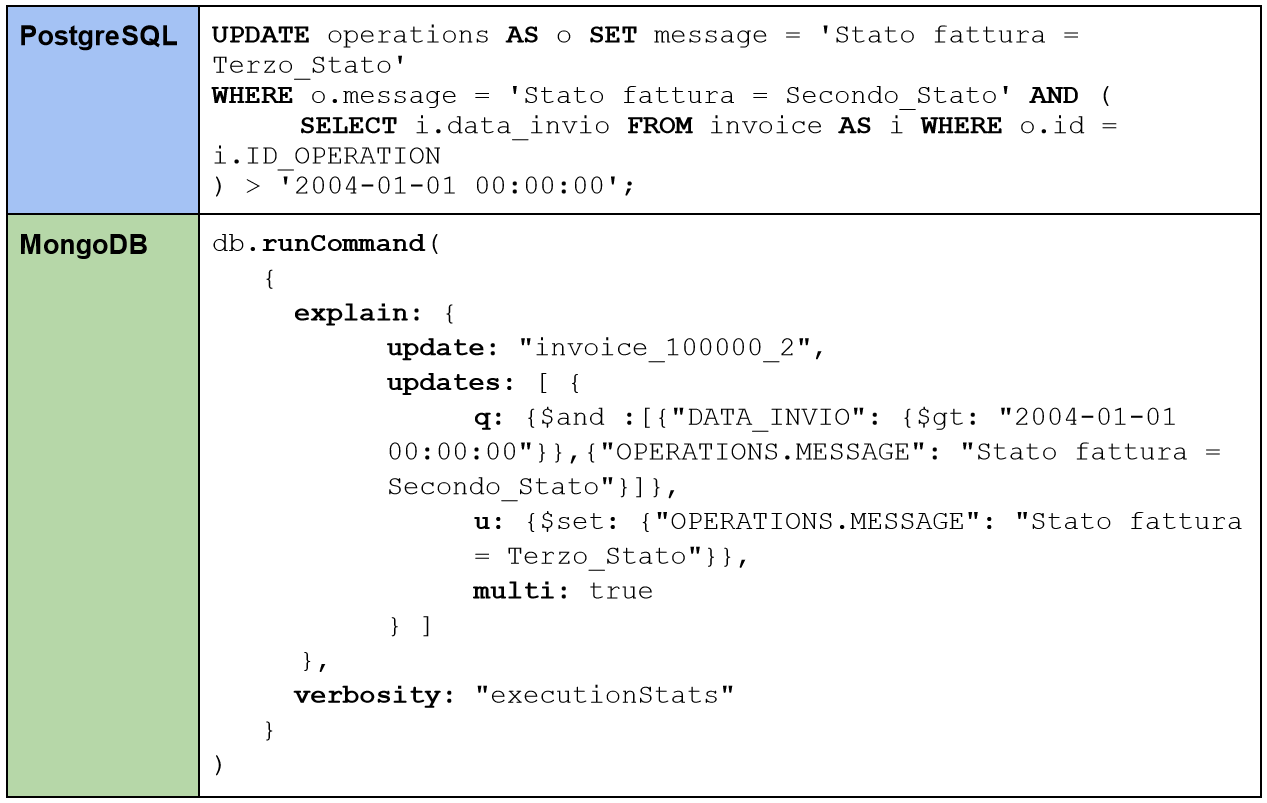
\includegraphics[height=22em]{immagini/query/query6.png}
\caption{Codice della query numero 6, scritto in entrambi i linguaggi}
\label{fig:query6}
\end{center}
\end{figure}

\noindent La query su PostgreSQL impiega dai 2 ai 5 minuti per essere portata a termine su un database contenente 100.000 elementi.\\
Osservando la \autoref{tab:query6}, presa direttamente da pgAdmin, possiamo notare come quasi tutto questo tempo sia utilizzato per effettuare uno scan della tabella \texttt{OPERATIONS}, che viene poi aggiornata.\\

\begin{table}
\begin{center} 
    \renewcommand{\arraystretch}{1.5}
    
    \centering
    \begin{longtable}{| C{2.5cm} | C{4cm} | C{4cm} |}
        
        \hline
        
        \rowcolor{mongogreen}
        \textbf{Node type} & \textbf{Count} & \textbf{Time spent} \\
        
        \hline
        Sequence Scan & 2 & 141140.886 ms \\
        \hline 
        Update & 1 & 322.887 ms \\
        \hline
        
        \caption{Estratto di tabella sui tempi di esecuzione della query numero 6 in pgAdmin}
        \label{tab:query6}
    \end{longtable}
\end{center}
\end{table}

\noindent MongoDB impiega soltanto 65 millisecondi per effettuare tutte le operazioni.\\
Ripetendo la query su database più ampi il risultato non cambia. Per 250.000 elementi PostgreSQL impiega più di trenta minuti, MongoDB si mantiene sotto i 200 millisecondi. Il tempo raddoppia quando all'interno del database sono contenuti 500.000 elementi. Per questa quantità di dati, PostgreSQL non restituisce un risultato in tempi utili.\\

%--------------------------------------------------------------

\subsection{Query 7}
La query riportata in \autoref{fig:query7} rappresenta un altro caso d'uso importante.

\begin{figure}[htbp]
\begin{center}
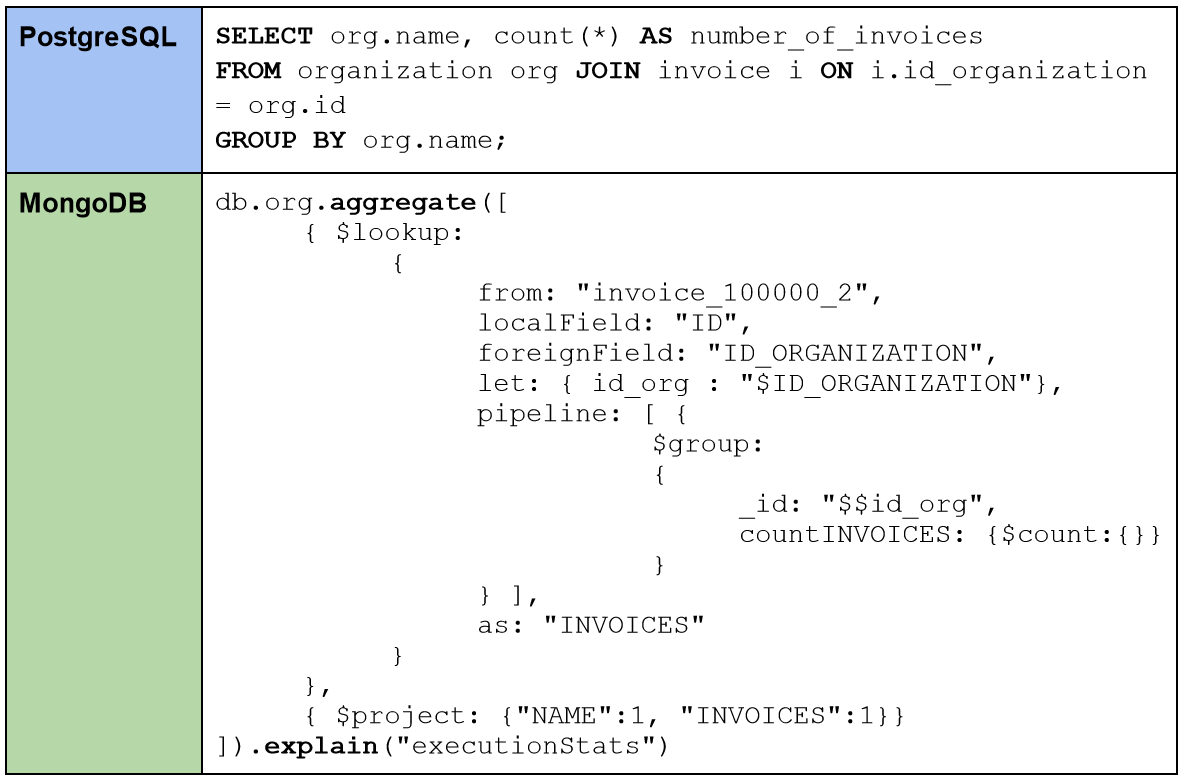
\includegraphics[height=22em]{immagini/query/query7.png}
\caption{Codice della query numero 7, scritto in entrambi i linguaggi}
\label{fig:query7}
\end{center}
\end{figure}

\noindent Come già menzionato, MongoDB è sì un database NoSQL, ma tecnicamente è considerabile anche ``relazionale'', perchè consente di effettuare operazioni di \textit{lookup} tra \textit{collection} diverse per unire informazioni altrimenti separate. Questa, tuttavia, non è sicuramente la feature di punta di un database documentale, e si traduce quindi in un'operazione piuttosto lenta rispetto ad altre operazioni per cui un un database di questo tipo è stato espressamente studiato.\\

\noindent Tutto questo è dimostrato dai dati statistici raccolti durante l'esecuzione delle query e riportati in \autoref{fig:query7.2}.\\
Per PostgreSQL si tratta di una join piuttosto semplice, accoppiata ad un raggruppamento. Il tempo di esecuzione si aggira intorno ai 65 ms se le tabelle \texttt{INVOICE} e \texttt{ORGANIZATION} contengono 100.000 elementi ciascuna.\\
MongoDB impiega tra i 5 e i 6 secondi per la stessa operazione, con la stessa quantità di dati.

\begin{figure}[htbp]
\begin{center}
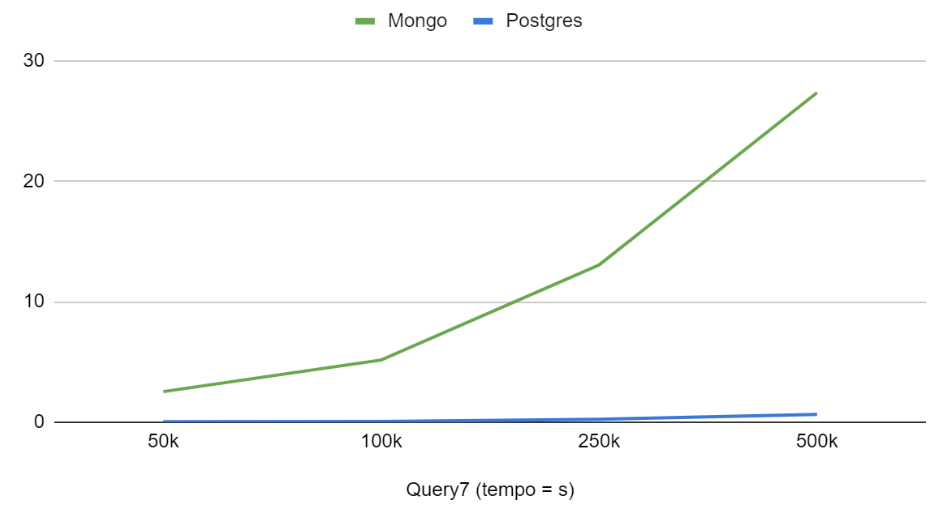
\includegraphics[height=15em]{immagini/query/query7_results.png}
\caption{Risultato del confronto, query numero 7}
\label{fig:query7.2}
\end{center}
\end{figure}

\noindent Con questa query si conclude la fase di confronto diretto tra i tempi di esecuzione delle operazioni sui due database. Vale la pena di evidenziare un fattore che sicuramente salta all'occhio leggendo le precedenti pagine: la complessità del linguaggio utilizzato per le query di MongoDB non è trascurabile e rispetto all'immediatezza di \gls{SQL}\ped{G} risulta piuttosto impegnativo da imparare, utilizzare e comprendere.

%**************************************************************
\section{Inserimento della fattura integrale}
\label{sec:fattura-integrale}
Uno dei casi d'uso di interesse per l'analisi condotta su \textit{InvoiceChannel} è quello che riguarda il salvataggio delle fatture.\\
Sebbene parte dei dati che le compongono sia salvata nella tabella invoice, per velocizzare l'accesso alle informazioni più importanti la fattura viene anche salvata per intero in formato \texttt{XML}.\\

\noindent Questo ovviamente non può essere fatto all'interno del database, principalmente perchè salvare una così grande quantità di dati all'interno di un unico campo non è desiderabile.\\
All'estremo opposto c'è la possibilità di elaborare il contenuto del file per scomporlo in campi salvabili e indicizzabili, potendo così ricomporre la fattura quando necessario. Anche questa soluzione presenta delle criticità, perchè effettuare operazioni di questo tipo su ogni fattura introdotta nel sistema creerebbe probabilmente un collo di bottiglia, e anche ricomporla quando necessario potrebbe rivelarsi costoso o non pratico.\\

\noindent La soluzione, come spesso succede, sta nel mezzo, e se ne trova un esempio all'interno dell'architettura di MongoDB, come di seguito riportato.\\
Come è stato visto, MongoDB salva i propri documenti in formato \texttt{JSON}, introducendo degli ``effetti collaterali'' che tornano utili al nostro caso d'uso.\\
L'idea è di convertire le fatture da \texttt{XML} a \texttt{JSON} per poi salvarle integralmente all'interno di una collection apposita.\\
In questo modo la fattura sarebbe sempre a disposizione per intero all'interno del database, come se fosse stato inserito il file \texttt{XML} in un campo di tabella. Allo stesso tempo sarebbe facile effettuare ricerche sui ``campi'' che compongono la fattura, per natura stessa dei file \texttt{JSON}, senza dover fare alcuna operazione di scomposizione e ricostruzione del file, se non per l'iniziale traduzione da un formato all'altro.\\

\noindent Tale trasformazione è bidirezionale, quindi così come si è passati dall'\texttt{XML} al \texttt{JSON} si può fare il contrario senza alcuna perdita di dati. Questo è importante perchè a livello legale \texttt{XML} rimane il formato ufficiale per le fatture elettroniche, quindi in caso di necessità si può ricostruire l'originale.\\

\noindent Tutto questo ovviamente ha un costo, e sta a chi crea un sistema di questo tipo il compito di soppesare pro e contro. MongoDB supporta l'inserimento di file \texttt{BSON} fino a 16 MB e una fattura tradotta in formato \texttt{JSON} occupa circa 5 KB, quindi sebbene appaia come un file ``grande'' all'occhio umano, si tratta di una dimensione bel al di sotto dei limiti strutturali del database. Le prestazioni non sarebbero intaccate da questo tipo di soluzione, anche quando si considera l'archiviazione di centinaia di migliaia di fatture, specialmente se si fa uso di indici.\\
Anche il costo della traduzione da \texttt{XML} a \texttt{JSON} va sicuramente rendicontato, ma dai test condotti non sembra avere un grosso impatto. Utilizzando uno strumento esterno basato su \gls{npm}\ped{G} è possibile automatizzare questo processo ad un bassissimo costo computazionale\cite{site:xml-js}.\\

\noindent Si conclude quindi che l'implementazione di una soluzione ibrida potrebbe portare miglioramenti prestazionali per quanto riguarda la consultazione di fatture elettroniche all'interno dei software dell'azienda. Questo approccio incrementale potrebbe inoltre permettere ai team di sviluppo di familiarizzare con la nuova tecnologia in maniera graduale, permettendone l'assorbimento all'interno dello stack aziendale senza subire un rallentamento eccessivo nella produzione.
             % Product Design Freeze e SOP
%% !TEX encoding = UTF-8
% !TEX TS-program = pdflatex
% !TEX root = ../tesi.tex

%**************************************************************
\chapter{Conclusioni}
\label{cap:conclusioni}
%**************************************************************
\section{Risultati generali del confronto tra database}
Prima di avviare questo progetto di tesi è stata effettuata una breve ricerca per comprendere se l'argomento fosse stato già esplorato in precedenza in altri contesti.\\
Sono state individuate altre tesi dai temi simili che propongono il confronto all'interno di database ``da laboratorio'', e alcune ricerche condotte su larga scala da aziende.\\
Vista la natura di questo progetto, legato ai prodotti software sviluppati da Ifin Sistemi, la prospettiva di effettuare una ricerca approfondita risultava comunque interessante.\\

\noindent Le conclusioni raggiunte al termine dei due mesi di tirocinio non sono dissimili da quelle raggiunte da altre ricerche, come ad esempio quelle svolte da OnGres, quando queste sono state condotte senza lo scopo di pubblicizzare l'una o l'altra tecnologia.\\
Come in molti altri ambiti, anche in questo caso il contesto di utilizzo di uno strumento ne determina efficacia ed efficienza.\\
L'introduzione dei database NoSQL ha permesso di raggiungere risultati estremamente vantaggiosi in molti ambiti applicativi, ma questo non li rende uno strumento universale per potenziare qualsiasi database in ogni contesto.\\
Tale fatto è valido per qualsiasi tecnologia, ma lo è ancora di più quando si parla di database NoSQL, data la grande varietà di soluzioni che questo gruppo comprende.\\
Nel caso specifico di MongoDB è facile essere tentati di farne largo uso in molti contesti diversi, grazie alla sua versatilità, semplicità e alla grande disponibilità di documentazione e risorse, data la sua natura \textit{open source}.\\
Si è visto tuttavia come in determinati casi questa potrebbe non essere la scelta migliore.\\
Allo stesso tempo, fare affidamento solo alle tecnologie già consolidate, con alle spalle anni di sviluppo e di esperienza, può ancorare il proprio software a delle soluzioni vecchie o inadeguate.\\

\noindent Anche in questo caso, la soluzione migliore deriva da un compromesso. L'utilizzo di database ibridi che permettono di sfruttare il meglio di entrambe le tecnologie può garantire migliori prestazioni senza sacrificare solidità delle strutture e affidabilità del servizio.\\


%**************************************************************
\section{Risultati specifici per il contesto di Ifin Sistemi}
Per quanto riguarda l'azienda per cui è stato condotto lo studio e il software su cui è stato basato, i risultati suggeriscono l'implementazione di una soluzione ibrida, che potrebbe migliorare il software, alleggerendo il carico di lavoro per i database tradizionali e permettendo di implementare nuove funzionalità.\\

\noindent Non è tuttavia prevista, nell'immediato futuro, un'analisi più approfondita volta a provare quanto postulato con questa tesi, per rendere più realistica l'idea di una migrazione di database. Come già evidenziato dal dialogo avuto con i team dedicati allo sviluppo dei software analizzati, le soluzioni adottate fin'ora per potenziare i database in uso sono state al contempo dispendiose da implementare (a livello di tempo ed energia) e proficue nel modo in cui sono riuscite a tamponare i problemi di disponibilità a cui tali tecnologie sono andate incontro con l'aumentare del carico di lavoro imposto.\\
Finchè i sistemi adottati continuano a funzionare stabilmente, non ha senso per l'azienda dedicare forza lavoro allo studio di nuove tecnologie, soprattutto in luce di un secondo fattore estremamente centrale: i prodotti dell'azienda non sono nuovi. Questo ha un peso per quel che riguarda la necessità di far ``collaborare'' tecnologie nuove con altre meno recenti, ma significa soprattutto che negli anni in cui LegalArchive e InvoiceChannel (i prodotti in questione) sono stati in commercio, il naturale ciclo di manutenzione e upgrade del software ha avuto corso, rendendoli dei progetti estremamente grandi e complessi, la cui migrazione richiederebbe probabilmente più energie di quelle che si andrebbero a risparmiare una volta terminata.\\

\noindent Ciò che questa ricerca può aspirare ad essere è uno spunto per evidenziare quanto l'implementazione ibrida di soluzioni relazionali miste a quelle NoSQL possa essere proficua. La soluzione che viene proposta nella \autoref{sec:fattura-integrale} è un esempio valido di questa convivenza di tecnologie, e rappresenta un buon punto di partenza qualora l'azienda decidesse di percorrere questa strada.\\


%**************************************************************
\section{Conoscenze acquisite e valutazione personale}
Il progetto di tirocinio mi aveva inizialmente attirato per la prospettiva di riprendere in mano le consocenze acquisite nell'ambito delle basi di dati ed approfondirle entrando a contatto con tecnologie più nuove, in grado di mettere in discussione i paradigmi su cui ci si basa quando si approccia per la prima volta questo contesto.\\

\noindent Le mie aspettative sono state soddisfatte ampiamente, sia per quanto riguarda la possibilità di eseguire degli studi su quello che è lo stato dell'arte ad oggi nell'ambito NoSQL, ma anche per le possibilità che ho avuto di sviluppare qualcosa di più concreto e potenzialmente utile, sia per me che per l'azienda.\\

\noindent È stato inoltre estremamente interessante ed importante per me avere la possibilità di approcciarmi all'ambiente lavorativo, in cui ho potuto imparare a muovermi seguendo ritmi e direttive diverse da quelle a cui ci si abitua all'interno dell'Università.\\

\noindent La concomitanza di tutte queste condizioni ha reso questo stage un'esperienza proficua e nel complesso positiva.\\
             % Conclusioni
\appendix                               
% !TEX encoding = UTF-8
% !TEX TS-program = pdflatex
% !TEX root = ../tesi.tex

%**************************************************************
\chapter{Appendice A}
%**************************************************************

\epigraph{Citazione}{Autore della citazione}



             % Appendice A

%**************************************************************
% Materiale finale
%**************************************************************
\backmatter
\printglossary[type=\acronymtype, title=Acronimi e abbreviazioni, toctitle=Acronimi e abbreviazioni]
\printglossary[type=main, title=Glossario, toctitle=Glossario]
% !TEX encoding = UTF-8
% !TEX TS-program = pdflatex
% !TEX root = ../tesi.tex

%**************************************************************
% Bibliografia
%**************************************************************

\cleardoublepage
\chapter{Bibliografia}

\nocite{*}

% Stampa i siti web consultati
\printbibliography[heading=subbibliography,title={Siti web consultati},type=online]


\end{document}
